\documentclass[10pt]{article}
\usepackage[utf8]{inputenc}
\usepackage[T1]{fontenc}
\usepackage{amsmath}
\usepackage{amsfonts}
\usepackage{amssymb}
\usepackage{mhchem}
\usepackage{stmaryrd}
\usepackage{bbold}
\usepackage{graphicx}
\usepackage[export]{adjustbox}
\graphicspath{ {./images/} }

\title{Chapter 11 }

\author{}
\date{}


\begin{document}
\maketitle
\section{Multivariate Regression}
\subsection{Introduction}
Multivariate regression is a system of regression equations. Multivariate regression is used as reduced form models for instrumental variable estimation (Chaper 12), vector autoregressions (Chapter 15), demand systems (demand for multiple goods), and other contexts.

Multivariate regression is also called by the name systems of regression equations. Closely related is the method of Seemingly Unrelated Regressions (SUR) introduced in Section 11.7.

Most of the tools of single equation regression generalize to multivariate regression. A major difference is a new set of notation to handle matrix estimators.

\subsection{Regression Systems}
A univariate linear regression equation equals $Y=X^{\prime} \beta+e$ where $Y$ is scalar and $X$ is a vector. Multivariate regression is a system of $m$ linear regressions, and equals
$$
Y_{j}=X_{j}^{\prime} \beta_{j}+e_{j}
$$
for $j=1, \ldots, m$. Here we use the subscript $j$ to denote the $j^{t h}$ dependent variable, not the $i^{t h}$ individual. As an example, $Y_{j}$ could be expenditures by a household on good category $j$ (e.g., food, housing, transportation, clothing, recreation). The regressor vectors $X_{j}$ are $k_{j} \times 1$ and $e_{j}$ is an error. The coefficient vectors $\beta_{j}$ are $k_{j} \times 1$. The total number of coefficients are $\bar{k}=\sum_{j=1}^{m} k_{j}$. The regressors can be common across $j$ or can vary across $j$. In the household expenditure example the regressors $X_{j}$ are typically common across $j$, and include variables such as household income, number and ages of family members, and demographic characteristics. The regression system specializes to univariate regression when $m=1$.

Define the $m \times 1$ error vector $e=\left(e_{1}, \ldots, e_{m}\right)^{\prime}$ and its $m \times m$ covariance matrix $\Sigma=\mathbb{E}\left[e e^{\prime}\right]$. The diagonal elements are the variances of the errors $e_{j}$ and the off-diagonals are the covariances across variables.

We can group the $m$ equations (11.1) into a single equation as follows. Let $Y=\left(Y_{1}, \ldots, Y_{m}\right)^{\prime}$ be the $m \times 1$ vector of dependent variables. Define the $m \times \bar{k}$ matrix of regressors
$$
\bar{X}=\left(\begin{array}{cccc}
X_{1}^{\prime} & 0 & \cdots & 0 \\
\vdots & X_{2}^{\prime} & & \vdots \\
0 & 0 & \cdots & X_{m}^{\prime}
\end{array}\right)
$$
and the $\bar{k} \times 1$ stacked coefficient vector
$$
\beta=\left(\begin{array}{c}
\beta_{1} \\
\vdots \\
\beta_{m}
\end{array}\right)
$$
The $m$ regression equations can be jointly written as
$$
Y=\bar{X} \beta+e .
$$
This is a system of $m$ equations.

For $n$ observations the joint system can be written in matrix notation by stacking. Define
$$
\boldsymbol{Y}=\left(\begin{array}{c}
Y_{1} \\
\vdots \\
Y_{n}
\end{array}\right), \quad \boldsymbol{e}=\left(\begin{array}{c}
e_{1} \\
\vdots \\
e_{n}
\end{array}\right), \quad \overline{\boldsymbol{X}}=\left(\begin{array}{c}
\bar{X}_{1} \\
\vdots \\
\bar{X}_{n}
\end{array}\right)
$$
which are $m n \times 1, m n \times 1$, and $m n \times \bar{k}$, respectively. The system can be written as $\boldsymbol{Y}=\overline{\boldsymbol{X}} \beta+\boldsymbol{e}$.

In many applications the regressor vectors $X_{j}$ are common across the variables $j$, so $X_{j}=X$ and $k_{j}=k$. By this we mean that the same variables enter each equation with no exclusion restrictions. Several important simplifications occur in this context. One is that we can write (11.2) using the notation
$$
Y=\boldsymbol{B}^{\prime} X+e
$$
where $\boldsymbol{B}=\left(\beta_{1}, \beta_{2}, \cdots, \beta_{m}\right)$ is $k \times m$. Another is that we can write the joint system of observations in the $n \times m$ matrix notation $\boldsymbol{Y}=\boldsymbol{X} \boldsymbol{B}+\boldsymbol{E}$ where
$$
\boldsymbol{Y}=\left(\begin{array}{c}
Y_{1}^{\prime} \\
\vdots \\
Y_{n}^{\prime}
\end{array}\right), \quad \boldsymbol{E}=\left(\begin{array}{c}
e_{1}^{\prime} \\
\vdots \\
e_{n}^{\prime}
\end{array}\right), \quad \boldsymbol{X}=\left(\begin{array}{c}
X_{1}^{\prime} \\
\vdots \\
X_{n}^{\prime}
\end{array}\right)
$$
Another convenient implication of common regressors is that we have the simplification
$$
\bar{X}=\left(\begin{array}{cccc}
X^{\prime} & 0 & \cdots & 0 \\
0 & X^{\prime} & & 0 \\
\vdots & \vdots & & \vdots \\
0 & 0 & \cdots & X^{\prime}
\end{array}\right)=\boldsymbol{I}_{m} \otimes X^{\prime}
$$
where $\otimes$ is the Kronecker product (see Appendix A.21).

\section{$11.3$ Least Squares Estimator}
The equations (11.1) can be estimated by least squares. This takes the form
$$
\widehat{\beta}_{j}=\left(\sum_{i=1}^{n} X_{j i} X_{j i}^{\prime}\right)^{-1}\left(\sum_{i=1}^{n} X_{j i} Y_{j i}\right) .
$$
An estimator of $\beta$ is the stacked vector
$$
\widehat{\beta}=\left(\begin{array}{c}
\widehat{\beta}_{1} \\
\vdots \\
\widehat{\beta}_{m}
\end{array}\right) .
$$
We can alternatively write this estimator using the systems notation
$$
\widehat{\beta}=\left(\overline{\boldsymbol{X}}^{\prime} \overline{\boldsymbol{X}}\right)^{-1}\left(\overline{\boldsymbol{X}}^{\prime} \boldsymbol{Y}\right)=\left(\sum_{i=1}^{n} \bar{X}_{i}^{\prime} \bar{X}_{i}\right)^{-1}\left(\sum_{i=1}^{n} \bar{X}_{i}^{\prime} Y_{i}\right)
$$
To see this, observe that
$$
\begin{aligned}
\overline{\boldsymbol{X}}^{\prime} \overline{\boldsymbol{X}} &=\left(\begin{array}{ccc}
\bar{X}_{1}^{\prime} & \cdots & \bar{X}_{n}^{\prime}
\end{array}\right)\left(\begin{array}{c}
\bar{X}_{1} \\
\vdots \\
\bar{X}_{n}
\end{array}\right) \\
&=\sum_{i=1}^{n} \bar{X}_{i}^{\prime} \bar{X}_{i} \\
&=\sum_{i=1}^{n}\left(\begin{array}{cccc}
X_{1 i} & 0 & \cdots & 0 \\
\vdots & X_{2 i} & & \vdots \\
0 & 0 & \cdots & X_{m i}
\end{array}\right)\left(\begin{array}{ccccc}
X_{1 i}^{\prime} & 0 & \cdots & 0 \\
\vdots & X_{2 i}^{\prime} & & \vdots \\
0 & 0 & \cdots & X_{m i}^{\prime}
\end{array}\right) \\
&=\left(\begin{array}{cccccc}
\sum_{i=1}^{n} X_{1 i} X_{1 i}^{\prime} & & 0 \\
\vdots & & \sum_{i=1}^{n} X_{2 i} X_{2 i}^{\prime} & & & \\
0 & & 0 & \cdots & \sum_{i=1}^{n} X_{m i} X_{m i}^{\prime}
\end{array}\right)
\end{aligned}
$$
and
$$
\begin{aligned}
\overline{\boldsymbol{X}}^{\prime} \boldsymbol{Y} &=\left(\begin{array}{ccc}
\bar{X}_{1}^{\prime} & \cdots & \bar{X}_{n}^{\prime}
\end{array}\right)\left(\begin{array}{c}
Y_{1} \\
\vdots \\
Y_{n}
\end{array}\right) \\
&=\sum_{i=1}^{n} \bar{X}_{i}^{\prime} Y_{i} \\
&=\sum_{i=1}^{n}\left(\begin{array}{cccc}
X_{1 i} & 0 & \cdots & 0 \\
\vdots & X_{2 i} & & \vdots \\
0 & 0 & \cdots & X_{m i}
\end{array}\right)\left(\begin{array}{c}
Y_{1 i} \\
\vdots \\
Y_{m i}
\end{array}\right) \\
&=\left(\begin{array}{c}
\sum_{i=1}^{n} X_{1 i} Y_{1 i} \\
\vdots \\
\sum_{i=1}^{n} X_{m i} Y_{m i}
\end{array}\right) .
\end{aligned}
$$
Hence
$$
\begin{aligned}
\left(\overline{\boldsymbol{X}}^{\prime} \overline{\boldsymbol{X}}\right)^{-1}\left(\overline{\boldsymbol{X}}^{\prime} \boldsymbol{Y}\right) &=\left(\sum_{i=1}^{n} \bar{X}_{i} \bar{X}_{i}^{\prime}\right)^{-1}\left(\sum_{i=1}^{n} \bar{X}_{i} Y_{i}\right) \\
&=\left(\begin{array}{c}
\left(\sum_{i=1}^{n} X_{1 i} X_{1 i}^{\prime}\right)^{-1}\left(\sum_{i=1}^{n} X_{1 i} Y_{1 i}\right) \\
\vdots \\
\left(\sum_{i=1}^{n} X_{m i} X_{m i}^{\prime}\right)^{-1}\left(\sum_{i=1}^{n} X_{m i} Y_{m i}\right)
\end{array}\right) \\
&=\widehat{\beta}
\end{aligned}
$$
as claimed. The $m \times 1$ residual vector for the $i^{t h}$ observation is $\widehat{e}_{i}=Y_{i}-\overline{\boldsymbol{X}}_{i}^{\prime} \widehat{\beta}$. The least squares estimator of the $m \times m$ error covariance matrix is
$$
\widehat{\Sigma}=\frac{1}{n} \sum_{i=1}^{n} \widehat{e}_{i} \widehat{e}_{i}^{\prime} .
$$
In the case of common regressors, the least squares coefficients can be written as
$$
\widehat{\beta}_{j}=\left(\sum_{i=1}^{n} X_{i} X_{i}^{\prime}\right)^{-1}\left(\sum_{i=1}^{n} X_{i} Y_{j i}\right)
$$
and
$$
\widehat{\boldsymbol{B}}=\left(\widehat{\beta}_{1}, \widehat{\beta}_{2}, \cdots, \widehat{\beta}_{m}\right)=\left(\boldsymbol{X}^{\prime} \boldsymbol{X}\right)^{-1}\left(\boldsymbol{X}^{\prime} \boldsymbol{Y}\right) .
$$
In Stata, multivariate regression can be implemented using the mvreg command.

\subsection{Expectation and Variance of Systems Least Squares}
We can calculate the finite-sample expectation and variance of $\widehat{\beta}$ under the conditional expectation assumption
$$
\mathbb{E}[e \mid X]=0
$$
where $X$ is the union of the regressors $X_{j}$. Equation (11.7) is equivalent to $\mathbb{E}\left\lfloor Y_{j} \mid X\right\rfloor=X_{j}^{\prime} \beta_{j}$, which means that the regression model is correctly specified.

We can center the estimator as
$$
\widehat{\beta}-\beta=\left(\overline{\boldsymbol{X}}^{\prime} \overline{\boldsymbol{X}}\right)^{-1}\left(\overline{\boldsymbol{X}}^{\prime} \boldsymbol{e}\right)=\left(\sum_{i=1}^{n} \bar{X}_{i}^{\prime} \bar{X}_{i}\right)^{-1}\left(\sum_{i=1}^{n} \bar{X}_{i}^{\prime} e_{i}\right)
$$
Taking conditional expectations we find $\mathbb{E}[\widehat{\beta} \mid \boldsymbol{X}]=\beta$. Consequently, systems least squares is unbiased under correct specification.

To compute the variance of the estimator, define the conditional covariance matrix of the errors of the $i^{t h}$ observation $\mathbb{E}\left[e_{i} e_{i}^{\prime} \mid X_{i}\right]=\Sigma_{i}$ which in general is a function of $X_{i}$. If the observations are mutually independent then
$$
\mathbb{E}\left[\boldsymbol{e} \boldsymbol{e}^{\prime} \mid \boldsymbol{X}\right]=\mathbb{E}\left[\left(\begin{array}{cccc}
e_{1} e_{1}^{\prime} & e_{1} e_{2}^{\prime} & \cdots & e_{1} e_{n}^{\prime} \\
\vdots & \ddots & & \vdots \\
e_{n} e_{1}^{\prime} & e_{n} e_{2}^{\prime} & \cdots & e_{n} e_{n}^{\prime}
\end{array}\right) \mid \boldsymbol{X}\right]=\left(\begin{array}{cccc}
\Sigma_{1} & 0 & \cdots & 0 \\
\vdots & \ddots & & \vdots \\
0 & 0 & \cdots & \Sigma_{n}
\end{array}\right) \text {. }
$$
Also, by independence across observations,
$$
\operatorname{var}\left[\sum_{i=1}^{n} \bar{X}_{i}^{\prime} e_{i} \mid \boldsymbol{X}\right]=\sum_{i=1}^{n} \operatorname{var}\left[\bar{X}_{i}^{\prime} e_{i} \mid X_{i}\right]=\sum_{i=1}^{n} \bar{X}_{i}^{\prime} \Sigma_{i} \bar{X}_{i} .
$$
It follows that
$$
\operatorname{var}[\widehat{\beta} \mid \boldsymbol{X}]=\left(\overline{\boldsymbol{X}}^{\prime} \overline{\boldsymbol{X}}\right)^{-1}\left(\sum_{i=1}^{n} \bar{X}_{i}^{\prime} \Sigma_{i} \bar{X}_{i}\right)\left(\overline{\boldsymbol{X}}^{\prime} \overline{\boldsymbol{X}}\right)^{-1} .
$$
When the regressors are common so that $\bar{X}_{i}=\boldsymbol{I}_{m} \otimes X_{i}^{\prime}$ then the covariance matrix can be written as
$$
\operatorname{var}[\widehat{\beta} \mid \boldsymbol{X}]=\left(\boldsymbol{I}_{m} \otimes\left(\boldsymbol{X}^{\prime} \boldsymbol{X}\right)^{-1}\right)\left(\sum_{i=1}^{n}\left(\Sigma_{i} \otimes X_{i} X_{i}^{\prime}\right)\right)\left(\boldsymbol{I}_{m} \otimes\left(\boldsymbol{X}^{\prime} \boldsymbol{X}\right)^{-1}\right)
$$
If the errors are conditionally homoskedastic
$$
\mathbb{E}\left[e e^{\prime} \mid X\right]=\Sigma
$$
then the covariance matrix simplifies to
$$
\operatorname{var}[\widehat{\beta} \mid \boldsymbol{X}]=\left(\overline{\boldsymbol{X}}^{\prime} \overline{\boldsymbol{X}}\right)^{-1}\left(\sum_{i=1}^{n} \bar{X}_{i}^{\prime} \Sigma \bar{X}_{i}\right)\left(\overline{\boldsymbol{X}}^{\prime} \overline{\boldsymbol{X}}\right)^{-1}
$$
If both simplifications (common regressors and conditional homoskedasticity) hold then we have the considerable simplication
$$
\operatorname{var}[\widehat{\beta} \mid \boldsymbol{X}]=\Sigma \otimes\left(\boldsymbol{X}^{\prime} \boldsymbol{X}\right)^{-1} .
$$

\subsection{Asymptotic Distribution}
For an asymptotic distribution it is sufficient to consider the equation-by-equation projection model in which case
$$
\mathbb{E}\left[X_{j} e_{j}\right]=0 .
$$
First, consider consistency. Since $\widehat{\beta}_{j}$ are the standard least squares estimators, they are consistent for the projection coefficients $\beta_{j}$.

Second, consider the asymptotic distribution. Our single equation theory implies that the $\widehat{\beta}_{j}$ are asymptotically normal. But this theory does not provide a joint distribution of the $\widehat{\beta}_{j}$ across $j$, which we now derive. Since the vector
$$
\bar{X}_{i}^{\prime} e_{i}=\left(\begin{array}{c}
X_{1 i} e_{1 i} \\
\vdots \\
X_{m i} e_{m i}
\end{array}\right)
$$
is i.i.d. across $i$ and mean zero under (11.9), the central limit theorem implies
$$
\frac{1}{\sqrt{n}} \sum_{i=1}^{n} \bar{X}_{i}^{\prime} e_{i} \underset{d}{\longrightarrow} \mathrm{N}(0, \Omega)
$$
where
$$
\Omega=\mathbb{E}\left[\bar{X}_{i}^{\prime} e_{i} e_{i}^{\prime} \bar{X}_{i}\right]=\mathbb{E}\left[\bar{X}_{i}^{\prime} \Sigma_{i} \bar{X}_{i}\right] .
$$
The matrix $\Omega$ is the covariance matrix of the variables $X_{j i} e_{j i}$ across equations. Under conditional homoskedasticity (11.8) the matrix $\Omega$ simplifies to
$$
\Omega=\mathbb{E}\left[\bar{X}_{i}^{\prime} \Sigma \bar{X}_{i}\right]
$$
(see Exercise 11.1). When the regressors are common it simplies to
$$
\Omega=\mathbb{E}\left[e e^{\prime} \otimes X X^{\prime}\right]
$$
(see Exercise 11.2). Under both conditions (homoskedasticity and common regressors) it simplifies to
$$
\Omega=\Sigma \otimes \mathbb{E}\left[X X^{\prime}\right]
$$
(see Exercise 11.3).

Applied to the centered and normalized estimator we obtain the asymptotic distribution. Theorem 11.1 Under Assumption 7.2, $\sqrt{n}(\widehat{\beta}-\beta) \underset{d}{\longrightarrow} \mathrm{N}\left(0, \boldsymbol{V}_{\beta}\right)$ where $\boldsymbol{V}_{\beta}=$ $Q^{-1} \Omega Q^{-1}$ and
$$
\boldsymbol{Q}=\mathbb{E}\left[\bar{X}^{\prime} \bar{X}\right]=\left(\begin{array}{cccc}
\mathbb{E}\left[X_{1} X_{1}^{\prime}\right] & 0 & \cdots & 0 \\
\vdots & \ddots & & \vdots \\
0 & 0 & \cdots & \mathbb{E}\left[X_{m} X_{m}^{\prime}\right]
\end{array}\right)
$$
For a proof, see Exercise 11.4.

When the regressors are common the matrix $\boldsymbol{Q}$ simplifies as
$$
\boldsymbol{Q}=\boldsymbol{I}_{m} \otimes \mathbb{E}\left[X X^{\prime}\right]
$$
(See Exercise 11.5).

If both the regressors are common and the errors are conditionally homoskedastic (11.8) then we have the simplification
$$
\boldsymbol{V}_{\beta}=\Sigma \otimes\left(\mathbb{E}\left[X X^{\prime}\right]\right)^{-1}
$$
(see Exercise 11.6).

Sometimes we are interested in parameters $\theta=r\left(\beta_{1}, \ldots, \beta_{m}\right)=r(\beta)$ which are functions of the coefficients from multiple equations. In this case the least squares estimator of $\theta$ is $\widehat{\theta}=r(\widehat{\beta})$. The asymptotic distribution of $\widehat{\theta}$ can be obtained from Theorem $11.1$ by the delta method.

Theorem 11.2 Under Assumptions $7.2$ and $7.3, \sqrt{n}(\widehat{\theta}-\theta) \underset{d}{\longrightarrow} \mathrm{N}\left(0, \boldsymbol{V}_{\theta}\right)$ where $\boldsymbol{V}_{\theta}=\boldsymbol{R}^{\prime} \boldsymbol{V}_{\beta} \boldsymbol{R}$ and $\boldsymbol{R}=\frac{\partial}{\partial \beta} r(\beta)^{\prime} .$

For a proof, see Exercise 11.7.

Theorem $11.2$ is an example where multivariate regression is fundamentally distinct from univariate regression. Only by treating least squares as a joint estimator can we obtain a distributional theory for a function of multiple equations. We can thereby construct standard errors, confidence intervals, and hypothesis tests.

\subsection{Covariance Matrix Estimation}
From the finite sample and asymptotic theory we can construct appropriate estimators for the variance of $\widehat{\beta}$. In the general case we have
$$
\widehat{\boldsymbol{V}}_{\widehat{\beta}}=\left(\overline{\boldsymbol{X}}^{\prime} \overline{\boldsymbol{X}}\right)^{-1}\left(\sum_{i=1}^{n} \bar{X}_{i}^{\prime} \widehat{e}_{i} \widehat{e}_{i}^{\prime} \bar{X}_{i}\right)\left(\overline{\boldsymbol{X}}^{\prime} \overline{\boldsymbol{X}}\right)^{-1} .
$$
Under conditional homoskedasticity (11.8) an appropriate estimator is
$$
\widehat{\boldsymbol{V}}_{\widehat{\beta}}^{0}=\left(\overline{\boldsymbol{X}}^{\prime} \overline{\boldsymbol{X}}\right)^{-1}\left(\sum_{i=1}^{n} \bar{X}_{i}^{\prime} \widehat{\Sigma}_{i}\right)\left(\overline{\boldsymbol{X}}^{\prime} \overline{\boldsymbol{X}}\right)^{-1} .
$$
When the regressors are common then these estimators equal
$$
\widehat{\boldsymbol{V}}_{\widehat{\beta}}=\left(\boldsymbol{I}_{m} \otimes\left(\boldsymbol{X}^{\prime} \boldsymbol{X}\right)^{-1}\right)\left(\sum_{i=1}^{n}\left(\widehat{e}_{i} \widehat{e}_{i}^{\prime} \otimes X_{i} X_{i}^{\prime}\right)\right)\left(\boldsymbol{I}_{m} \otimes\left(\boldsymbol{X}^{\prime} \boldsymbol{X}\right)^{-1}\right)
$$
and $\widehat{\boldsymbol{V}}_{\widehat{\beta}}^{0}=\widehat{\Sigma} \otimes\left(\boldsymbol{X}^{\prime} \boldsymbol{X}\right)^{-1}$, respectively.

Covariance matrix estimators for $\widehat{\theta}$ are found as
$$
\begin{aligned}
\widehat{\boldsymbol{V}}_{\widehat{\theta}} &=\widehat{\boldsymbol{R}}^{\prime} \widehat{\boldsymbol{V}}_{\widehat{\beta}} \widehat{\boldsymbol{R}} \\
\widehat{\boldsymbol{V}}_{\widehat{\theta}}^{0} &=\widehat{\boldsymbol{R}}^{\prime} \widehat{\boldsymbol{V}}_{\widehat{\beta}}^{0} \widehat{\boldsymbol{R}} \\
\widehat{\boldsymbol{R}} &=\frac{\partial}{\partial \beta} r(\widehat{\beta})^{\prime} .
\end{aligned}
$$
Theorem 11.3 Under Assumption 7.2, $n \widehat{\boldsymbol{V}}_{\widehat{\beta}} \underset{p}{\rightarrow} \boldsymbol{V}_{\beta}$ and $n \widehat{\boldsymbol{V}}_{\widehat{\beta}}^{0} \vec{p}^{0} \boldsymbol{V}_{\beta}^{0}$

For a proof, see Exercise 11.8.

\subsection{Seemingly Unrelated Regression}
Consider the systems regression model under the conditional expectation and homoskedasticity assumptions
$$
\begin{aligned}
Y &=\bar{X} \beta+e \\
\mathbb{E}[e \mid X] &=0 \\
\mathbb{E}\left[e e^{\prime} \mid X\right] &=\Sigma .
\end{aligned}
$$
Since the errors are correlated across equations we consider estimation by Generalized Least Squares (GLS). To derive the estimator, premultiply (11.15) by $\Sigma^{-1 / 2}$ so that the transformed error vector is i.i.d. with covariance matrix $\boldsymbol{I}_{m}$. Then apply least squares and rearrange to find
$$
\widehat{\beta}_{\mathrm{gls}}=\left(\sum_{i=1}^{n} \bar{X}_{i}^{\prime} \Sigma^{-1} \bar{X}_{i}\right)^{-1}\left(\sum_{i=1}^{n} \bar{X}_{i}^{\prime} \Sigma^{-1} Y_{i}\right)
$$
(see Exercise 11.9). Another approach is to take the vector representation
$$
\boldsymbol{Y}=\overline{\boldsymbol{X}} \beta+\boldsymbol{e}
$$
and calculate that the equation error $\boldsymbol{e}$ has variance $\mathbb{E}\left[\boldsymbol{e} \boldsymbol{e}^{\prime}\right]=\boldsymbol{I}_{n} \otimes \Sigma$. Premultiply the equation by $\boldsymbol{I}_{n} \otimes$ $\Sigma^{-1 / 2}$ so that the transformed error has covariance matrix $\boldsymbol{I}_{n m}$ and then apply least squares to find
$$
\widehat{\beta}_{\mathrm{gls}}=\left(\overline{\boldsymbol{X}}^{\prime}\left(\boldsymbol{I}_{n} \otimes \Sigma^{-1}\right) \overline{\boldsymbol{X}}\right)^{-1}\left(\overline{\boldsymbol{X}}^{\prime}\left(\boldsymbol{I}_{n} \otimes \Sigma^{-1}\right) \boldsymbol{Y}\right)
$$
(see Exercise 11.10). Expressions (11.16) and (11.17) are algebraically equivalent. To see the equivalence, observe that
$$
\begin{aligned}
\overline{\boldsymbol{X}}^{\prime}\left(\boldsymbol{I}_{n} \otimes \Sigma^{-1}\right) \overline{\boldsymbol{X}} &=\left(\begin{array}{lll}
\bar{X}_{1}^{\prime} & \cdots & \bar{X}_{n}^{\prime}
\end{array}\right)\left(\begin{array}{cccc}
\Sigma^{-1} & 0 & \cdots & 0 \\
\vdots & \Sigma^{-1} & & \vdots \\
0 & 0 & \cdots & \Sigma^{-1}
\end{array}\right)\left(\begin{array}{c}
\bar{X}_{1} \\
\vdots \\
\bar{X}_{n}
\end{array}\right) \\
&=\sum_{i=1}^{n} \bar{X}_{i}^{\prime} \Sigma^{-1} \bar{X}_{i}
\end{aligned}
$$
and
$$
\begin{aligned}
\overline{\boldsymbol{X}}^{\prime}\left(\boldsymbol{I}_{n} \otimes \Sigma^{-1}\right) \boldsymbol{Y} &=\left(\begin{array}{lll}
\bar{X}_{1}^{\prime} & \cdots & \bar{X}_{n}^{\prime}
\end{array}\right)\left(\begin{array}{cccc}
\Sigma^{-1} & 0 & \cdots & 0 \\
\vdots & \Sigma^{-1} & & \vdots \\
0 & 0 & \cdots & 0^{-1}
\end{array}\right)\left(\begin{array}{c}
Y_{1} \\
\vdots \\
Y_{n}
\end{array}\right) \\
&=\sum_{i=1}^{n} \bar{X}_{i}^{\prime} \Sigma^{-1} Y_{i} .
\end{aligned}
$$
Since $\Sigma$ is unknown it must be replaced by an estimator. Using $\widehat{\Sigma}$ from (11.5) we obtain a feasible GLS estimator.
$$
\begin{aligned}
\widehat{\beta}_{\mathrm{sur}} &=\left(\sum_{i=1}^{n} \bar{X}_{i}^{\prime} \widehat{\Sigma}^{-1} \bar{X}_{i}\right)^{-1}\left(\sum_{i=1}^{n} \bar{X}_{i}^{\prime} \widehat{\Sigma}^{-1} Y_{i}\right) \\
&=\left(\overline{\boldsymbol{X}}^{\prime}\left(\boldsymbol{I}_{n} \otimes \widehat{\Sigma}^{-1}\right) \overline{\boldsymbol{X}}\right)^{-1}\left(\overline{\boldsymbol{X}}^{\prime}\left(\boldsymbol{I}_{n} \otimes \widehat{\Sigma}^{-1}\right) \boldsymbol{Y}\right) .
\end{aligned}
$$
This is the Seemingly Unrelated Regression (SUR) estimator as introduced by Zellner (1962).

The estimator $\widehat{\Sigma}$ can be updated by calculating the SUR residuals $\widehat{e}_{i}=Y_{i}-\bar{X}_{i}^{\prime} \widehat{\beta}_{\text {sur }}$ and the covariance matrix estimator $\widehat{\Sigma}=\frac{1}{n} \sum_{i=1}^{n} \widehat{e}_{i} \widehat{e}_{i}^{\prime}$. Substituted into (11.18) we obtain an iterated SUR estimator. This can be iterated until convergence.

Under conditional homoskedasticity (11.8) we can derive its asymptotic distribution.

Theorem 11.4 Under Assumption $7.2$ and (11.8)
$$
\sqrt{n}\left(\widehat{\beta}_{\text {sur }}-\beta\right) \underset{d}{\longrightarrow} \mathrm{N}\left(0, V_{\beta}^{*}\right)
$$
where $\boldsymbol{V}_{\beta}^{*}=\left(\mathbb{E}\left[\bar{X}^{\prime} \Sigma^{-1} \bar{X}\right]\right)^{-1}$.

For a proof, see Exercise 11.11.

Under these assumptions, SUR is more efficient than least squares.

Theorem 11.5 Under Assumption $7.2$ and (11.8)
$$
\boldsymbol{V}_{\beta}^{*}=\left(\mathbb{E}\left[\bar{X}^{\prime} \Sigma^{-1} \bar{X}\right]\right)^{-1} \leq\left(\mathbb{E}\left[\bar{X}^{\prime} \bar{X}\right]\right)^{-1} \mathbb{E}\left[\bar{X}^{\prime} \Sigma \bar{X}\right]\left(\mathbb{E}\left[\bar{X}^{\prime} \bar{X}\right]\right)^{-1}=\boldsymbol{V}_{\beta}
$$
and thus $\widehat{\beta}_{\text {sur }}$ is asymptotically more efficient than $\widehat{\beta}_{\text {ols. }}$. For a proof, see Exercise 11.12.

An appropriate estimator of the variance of $\widehat{\beta}_{\text {sur }}$ is
$$
\widehat{\boldsymbol{V}}_{\widehat{\beta}}=\left(\sum_{i=1}^{n} \bar{X}_{i}^{\prime} \widehat{\Sigma}^{-1} \bar{X}_{i}\right)^{-1}
$$
Theorem 11.6 Under Assumption $7.2$ and (11.8) $n \widehat{\boldsymbol{V}}_{\widehat{\beta}} \underset{p}{\longrightarrow} \boldsymbol{V}_{\beta}$.

For a proof, see Exercise 11.13.

In Stata, the seemingly unrelated regressions estimator is implemented using the sureg command.

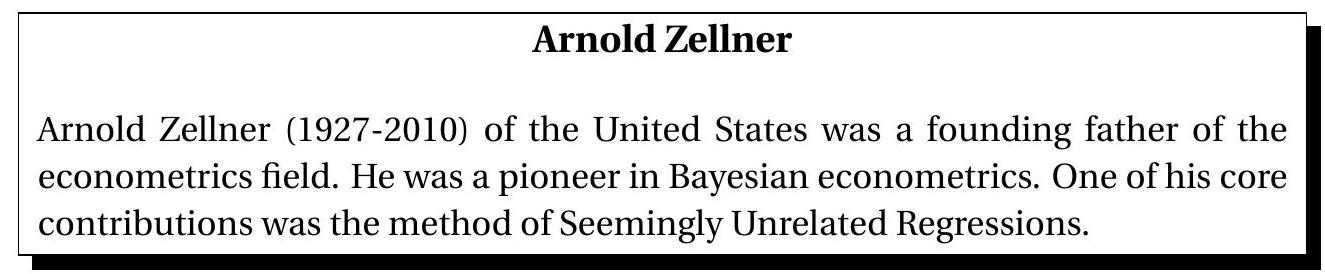
\includegraphics[max width=\textwidth]{2022_09_17_2536389c9af66f64c886g-09}

\subsection{Equivalence of SUR and Least Squares}
When the regressors are common across equations $X_{j}=X$ it turns out that the SUR estimator simplifies to least squares.

To see this, recall that when regressors are common this implies that $\bar{X}=\boldsymbol{I}_{m} \otimes X^{\prime}$. Then
$$
\begin{aligned}
\bar{X}_{i}^{\prime} \widehat{\Sigma}^{-1} &=\left(\boldsymbol{I}_{m} \otimes X_{i}\right) \widehat{\Sigma}^{-1} \\
&=\widehat{\Sigma}^{-1} \otimes X_{i} \\
&=\left(\widehat{\Sigma}^{-1} \otimes \boldsymbol{I}_{k}\right)\left(\boldsymbol{I}_{m} \otimes X_{i}\right) \\
&=\left(\widehat{\Sigma}^{-1} \otimes \boldsymbol{I}_{k}\right) \bar{X}_{i}^{\prime} .
\end{aligned}
$$
Thus
$$
\begin{aligned}
\widehat{\beta}_{\mathrm{sur}} &=\left(\sum_{i=1}^{n} \bar{X}_{i}^{\prime} \widehat{\Sigma}^{-1} \bar{X}_{i}\right)^{-1}\left(\sum_{i=1}^{n} \bar{X}_{i}^{\prime} \widehat{\Sigma}^{-1} Y_{i}\right) \\
&=\left(\left(\widehat{\Sigma}^{-1} \otimes \boldsymbol{I}_{k}\right) \sum_{i=1}^{n} \bar{X}_{i}^{\prime} \bar{X}_{i}\right)^{-1}\left(\left(\widehat{\Sigma}^{-1} \otimes \boldsymbol{I}_{k}\right) \sum_{i=1}^{n} \bar{X}_{i}^{\prime} Y_{i}\right) \\
&=\left(\sum_{i=1}^{n} \bar{X}_{i}^{\prime} \bar{X}_{i}\right)^{-1}\left(\sum_{i=1}^{n} \bar{X}_{i}^{\prime} Y_{i}\right)=\widehat{\beta}_{\mathrm{ols}}
\end{aligned}
$$
A model where regressors are not common across equations is nested within a model with the union of all regressors included in all equations. Thus the model with regressors common across equations is a fully unrestricted model, and a model where the regressors differ across equations is a restricted model. Thus the above result shows that the SUR estimator reduces to least squares in the absence of restrictions, but SUR can differ from least squares otherwise.

Another context where SUR=OLS is when the variance matrix is diagonal, $\Sigma=\operatorname{diag}\left\{\sigma_{1}^{2}, \ldots, \sigma_{m}^{2}\right\}$. In this case $\Sigma^{-1 / 2} \bar{X}_{i}=\bar{X}_{i} \operatorname{diag}\left\{\boldsymbol{I}_{k_{1}} \sigma_{1}^{-1 / 2}, \ldots, \boldsymbol{I}_{k_{m}} \sigma_{m}^{-1 / 2}\right\}$ from which you can calculate that $\widehat{\beta}_{\text {sur }}=\widehat{\beta}_{\text {ols }}$. The intuition is that there is no difference in systems estimation when the equations are uncorrelated, which occurs when $\Sigma$ is diagonal.

\subsection{Maximum Likelihood Estimator}
Take the linear model under the assumption that the error is independent of the regressors and multivariate normally distributed. Thus $Y=\bar{X} \beta+e$ with $e \sim \mathrm{N}(0, \Sigma)$. In this case we can consider the maximum likelihood estimator (MLE) of the coefficients.

It is convenient to reparameterize the covariance matrix in terms of its inverse $S=\Sigma^{-1}$. With this reparameterization the conditional density of $Y$ given $X=x$ equals
$$
f(y \mid x)=\frac{\operatorname{det}(\boldsymbol{S})^{1 / 2}}{(2 \pi)^{m / 2}} \exp \left(-\frac{1}{2}(y-x \beta)^{\prime} \boldsymbol{S}(y-x \beta)\right) .
$$
The log-likelihood function for the sample is
$$
\ell_{n}(\beta, \boldsymbol{S})=-\frac{n m}{2} \log (2 \pi)+\frac{n}{2} \log (\operatorname{det}(\boldsymbol{S}))-\frac{1}{2} \sum_{i=1}^{n}\left(Y_{i}-\bar{X}_{i} \beta\right)^{\prime} S\left(Y_{i}-\bar{X}_{i} \beta\right) .
$$
The maximum likelihood estimator $\left(\widehat{\beta}_{\text {mle }}, \widehat{S}_{\text {mle }}\right)$ maximizes the log-likelihood function. The first order conditions are
$$
0=\left.\frac{\partial}{\partial \beta} \ell_{n}(\beta, \boldsymbol{S})\right|_{\beta=\widehat{\beta}, \boldsymbol{S}=\widehat{\boldsymbol{S}}}=\sum_{i=1}^{n} \bar{X}_{i} \widehat{\boldsymbol{S}}\left(Y_{i}-\bar{X}_{i} \widehat{\beta}\right)
$$
and
$$
0=\left.\frac{\partial}{\partial \boldsymbol{S}} \ell_{n}(\beta, \Sigma)\right|_{\beta=\widehat{\beta}, \boldsymbol{S}=\widehat{\boldsymbol{S}}}=\frac{n}{2} \widehat{\boldsymbol{S}}^{-1}-\frac{1}{2} \operatorname{tr}\left(\sum_{i=1}^{n}\left(Y_{i}-\bar{X}_{i} \widehat{\beta}\right)\left(Y_{i}-\bar{X}_{i} \widehat{\beta}\right)^{\prime}\right)
$$
The second equation uses the matrix results $\frac{\partial}{\partial S} \log (\operatorname{det}(\boldsymbol{S}))=\boldsymbol{S}^{-1}$ and $\frac{\partial}{\partial \boldsymbol{B}} \operatorname{tr}(\boldsymbol{A B})=\boldsymbol{A}^{\prime}$ from Appendix A.20.

Solving and making the substitution $\widehat{\Sigma}=\widehat{\boldsymbol{S}}^{-1}$ we obtain
$$
\begin{gathered}
\widehat{\beta}_{\mathrm{mle}}=\left(\sum_{i=1}^{n} \bar{X}_{i}^{\prime} \widehat{\Sigma}^{-1} \bar{X}_{i}\right)^{-1}\left(\sum_{i=1}^{n} \bar{X}_{i}^{\prime} \widehat{\Sigma}^{-1} Y_{i}\right) \\
\widehat{\Sigma}_{\mathrm{mle}}=\frac{1}{n} \sum_{i=1}^{n}\left(Y_{i}-\bar{X}_{i} \widehat{\beta}\right)\left(Y_{i}-\bar{X}_{i} \widehat{\beta}\right)^{\prime} .
\end{gathered}
$$
Notice that each equation refers to the other. Hence these are not closed-form expressions but can be solved via iteration. The solution is identical to the iterated SUR estimator. Thus the iterated SUR estimator is identical to MLE under normality.

Recall that the SUR estimator simplifies to OLS when the regressors are common across equations. The same occurs for the MLE. Thus when $\bar{X}_{i}=\boldsymbol{I}_{m} \otimes X_{i}^{\prime}$ we find that $\widehat{\beta}_{\mathrm{mle}}=\widehat{\beta}_{\text {ols }}$ and $\widehat{\Sigma}_{\text {mle }}=\widehat{\Sigma}_{\text {ols }}$.

\subsection{Restricted Estimation}
In many multivariate regression applications it is desired to impose restrictions on the coefficients. In particular, cross-equation restrictions (for example, imposing Slutsky symmetry on a demand system) can be quite important and can only be imposed by a multivariate estimation method. Estimation subject to restrictions can be done by minimum distance, maximum likelihood, or the generalized method of moments.

Minimum distance is a straightforward application of the methods of Chapter 8 to the estimators presented in this chapter, as such methods apply to any asymptotically normal estimator.

Imposing restrictions on maximum likelihood is also straightforward. The likelihood is maximized subject to the imposed restrictions. One important example is explored in detail in the following section.

Generalized method of moments estimation of multivariate regression subject to restrictions will be explored in Section 13.18. This is a particularly simple and straightforward way to estimate restricted multivariate regression models and is our generally preferred approach.

\subsection{Reduced Rank Regression}
One context where systems estimation is important is when it is desired to impose or test restrictions across equations. Restricted systems are commonly estimated by maximum likelihood under normality. In this section we explore one important special case of restricted multivariate regression known as reduced rank regression. The model was originally proposed by Anderson (1951) and extended by Johansen (1995).

The unrestricted model is
$$
\begin{aligned}
Y &=\boldsymbol{B}^{\prime} X+\boldsymbol{C}^{\prime} Z+e \\
\mathbb{E}\left[e e^{\prime} \mid X, Z\right] &=\Sigma
\end{aligned}
$$
where $\boldsymbol{B}$ is $k \times m, \boldsymbol{C}$ is $\ell \times m, Y \in \mathbb{R}^{m}, X \in \mathbb{R}^{k}$, and $Z \in \mathbb{R}^{\ell}$. We separate the regressors as $X$ and $Z$ because the coefficient matrix $\boldsymbol{B}$ will be restricted while $\boldsymbol{C}$ will be unrestricted.

The matrix $\boldsymbol{B}$ is full rank if
$$
\operatorname{rank}(\boldsymbol{B})=\min (k, m) .
$$
The reduced rank restriction is $\operatorname{rank}(\boldsymbol{B})=r<\min (k, m)$ for some known $r$.

The reduced rank restriction implies that we can write the coefficient matrix $\boldsymbol{B}$ in the factored form $\boldsymbol{B}=\boldsymbol{G} \boldsymbol{A}^{\prime}$ where $\boldsymbol{A}$ is $m \times r$ and $\boldsymbol{G}$ is $k \times r$. This representation is not unique as we can replace $\boldsymbol{G}$ with $\boldsymbol{G} \boldsymbol{Q}$ and $\boldsymbol{A}$ with $\boldsymbol{A} \boldsymbol{Q}^{-1 \prime}$ for any invertible $\boldsymbol{Q}$ and the same relation holds. Identification therefore requires a normalization of the coefficients. A conventional normalization is $\boldsymbol{G}^{\prime} \boldsymbol{D} \boldsymbol{G}=\boldsymbol{I}_{r}$ for given $\boldsymbol{D}$.

Equivalently, the reduced rank restriction can be imposed by requiring that $\boldsymbol{B}$ satisfy the restriction $\boldsymbol{B} \boldsymbol{A}_{\perp}=\boldsymbol{G} \boldsymbol{A}^{\prime} \boldsymbol{A}_{\perp}=0$ for some $m \times(m-r)$ coefficient matrix $\boldsymbol{A}_{\perp}$. Since $\boldsymbol{G}$ is full rank this requires that $\boldsymbol{A}^{\prime} \boldsymbol{A}_{\perp}=0$, hence $\boldsymbol{A}_{\perp}$ is the orthogonal complement of $\boldsymbol{A}$. Note that $\boldsymbol{A}_{\perp}$ is not unique as it can be replaced by $\boldsymbol{A}_{\perp} \boldsymbol{Q}$ for any $(m-r) \times(m-r)$ invertible $\boldsymbol{Q}$. Thus if $\boldsymbol{A}_{\perp}$ is to be estimated it requires a normalization.

We discuss methods for estimation of $\boldsymbol{G}, \boldsymbol{A}, \Sigma, \boldsymbol{C}$, and $\boldsymbol{A}_{\perp}$. The standard approach is maximum likelihood under the assumption that $e \sim \mathrm{N}(0, \Sigma)$. The log-likelihood function for the sample is
$$
\begin{aligned}
\ell_{n}(\boldsymbol{G}, \boldsymbol{A}, \boldsymbol{C}, \Sigma) &=-\frac{n m}{2} \log (2 \pi)-\frac{n}{2} \log (\operatorname{det}(\Sigma)) \\
&-\frac{1}{2} \sum_{i=1}^{n}\left(Y_{i}-\boldsymbol{A} \boldsymbol{G}^{\prime} X_{i}-\boldsymbol{C}^{\prime} Z_{i}\right)^{\prime} \Sigma^{-1}\left(Y_{i}-\boldsymbol{A} \boldsymbol{G}^{\prime} X_{i}-\boldsymbol{C}^{\prime} Z_{i}\right) .
\end{aligned}
$$
Anderson (1951) derived the MLE by imposing the constraint $\boldsymbol{B} \boldsymbol{A}_{\perp}=0$ via the method of Lagrange multipliers. This turns out to be algebraically cumbersome.

Johansen (1995) instead proposed the following straightforward concentration method. Treating $\boldsymbol{G}$ as if it is known, maximize the log-likelihood with respect to the other parameters. Resubstituting these estimators we obtain the concentrated log-likelihood function with respect to $\boldsymbol{G}$. This can be maximized to find the MLE for $\boldsymbol{G}$. The other parameter estimators are then obtain by substitution. We now describe these steps in detail.

Given $\boldsymbol{G}$ the likelihood is a normal multivariate regression in the variables $\boldsymbol{G}^{\prime} X$ and $Z$, so the MLE for $\boldsymbol{A}, \boldsymbol{C}$ and $\Sigma$ are least squares. In particular, using the Frisch-Waugh-Lovell residual regression formula we can write the estimators for $\boldsymbol{A}$ and $\Sigma$ as
$$
\widehat{\boldsymbol{A}}(\boldsymbol{G})=\left(\widetilde{\boldsymbol{Y}}^{\prime} \widetilde{\boldsymbol{X}} \boldsymbol{G}\right)\left(\boldsymbol{G}^{\prime} \widetilde{\boldsymbol{X}}^{\prime} \widetilde{\boldsymbol{X}} \boldsymbol{G}\right)^{-1}
$$
and
$$
\widehat{\Sigma}(\boldsymbol{G})=\frac{1}{n}\left(\widetilde{\boldsymbol{Y}}^{\prime} \tilde{\boldsymbol{Y}}-\widetilde{\boldsymbol{Y}}^{\prime} \widetilde{\boldsymbol{X}} \boldsymbol{G}\left(\boldsymbol{G}^{\prime} \widetilde{\boldsymbol{X}}^{\prime} \widetilde{\boldsymbol{X}} \boldsymbol{G}\right)^{-1} \boldsymbol{G}^{\prime} \widetilde{\boldsymbol{X}}^{\prime} \widetilde{\boldsymbol{Y}}\right)
$$
where $\tilde{\boldsymbol{Y}}=\boldsymbol{Y}-\boldsymbol{Z}\left(\boldsymbol{Z}^{\prime} \boldsymbol{Z}\right)^{-1} \boldsymbol{Z}^{\prime} \boldsymbol{Y}$ and $\widetilde{\boldsymbol{X}}=\boldsymbol{X}-\boldsymbol{Z}\left(\boldsymbol{Z}^{\prime} \boldsymbol{Z}\right)^{-1} \boldsymbol{Z}^{\prime} \boldsymbol{X}$.

Substituting these estimators into the log-likelihood function we obtain the concentrated likelihood function, which is a function of $G$ only.
$$
\begin{aligned}
\widetilde{\ell}_{n}(\boldsymbol{G}) &=\ell_{n}(\boldsymbol{G}, \widehat{\boldsymbol{A}}(\boldsymbol{G}), \widehat{\boldsymbol{C}}(\boldsymbol{G}), \widehat{\Sigma}(\boldsymbol{G})) \\
&=\frac{m}{2}(n \log (2 \pi)-1)-\frac{n}{2} \log \left[\operatorname{det}\left(\widetilde{\boldsymbol{Y}}^{\prime} \widetilde{\boldsymbol{Y}}-\widetilde{\boldsymbol{Y}}^{\prime} \widetilde{\boldsymbol{X}} \boldsymbol{G}\left(\boldsymbol{G}^{\prime} \widetilde{\boldsymbol{X}}^{\prime} \widetilde{\boldsymbol{X}} \boldsymbol{G}\right)^{-1} \boldsymbol{G}^{\prime} \widetilde{\boldsymbol{X}}^{\prime} \widetilde{\boldsymbol{Y}}\right)\right] \\
&=\frac{m}{2}(n \log (2 \pi)-1)-\frac{n}{2} \log \left(\operatorname{det}\left(\widetilde{\boldsymbol{Y}}^{\prime} \widetilde{\boldsymbol{Y}}\right)\right)-\frac{n}{2} \log \left[\frac{\operatorname{det}\left(\boldsymbol{G}^{\prime}\left(\widetilde{\boldsymbol{X}}^{\prime} \widetilde{\boldsymbol{X}}-\widetilde{\boldsymbol{X}}^{\prime} \tilde{\boldsymbol{Y}}\left(\widetilde{\boldsymbol{Y}}^{\prime} \widetilde{\boldsymbol{Y}}\right)^{-1} \boldsymbol{Y}^{\prime} \widetilde{\boldsymbol{X}}\right) \boldsymbol{G}\right)}{\operatorname{det}\left(\boldsymbol{G}^{\prime} \widetilde{\boldsymbol{X}}^{\prime} \widetilde{\boldsymbol{X}} \boldsymbol{G}\right)} .\right.
\end{aligned}
$$
The third equality uses Theorem A.1.8. The MLE $\widehat{\boldsymbol{G}}$ for $\boldsymbol{G}$ is the maximizer of $\widetilde{\ell}_{n}(\boldsymbol{G})$, or equivalently equals
$$
\begin{aligned}
\widehat{\boldsymbol{G}} &=\underset{\boldsymbol{G}}{\operatorname{argmin}} \frac{\operatorname{det}\left(\boldsymbol{G}^{\prime}\left(\widetilde{\boldsymbol{X}}^{\prime} \widetilde{\boldsymbol{X}}-\widetilde{\boldsymbol{X}}^{\prime} \widetilde{\boldsymbol{Y}}\left(\tilde{\boldsymbol{Y}}^{\prime} \widetilde{\boldsymbol{Y}}\right)^{-1} \boldsymbol{Y}^{\prime} \tilde{\boldsymbol{X}}\right) \boldsymbol{G}\right)}{\operatorname{det}\left(\boldsymbol{G}^{\prime} \widetilde{\boldsymbol{X}}^{\prime} \widetilde{\boldsymbol{X}} \boldsymbol{G}\right)} \\
&=\underset{\boldsymbol{G}}{\operatorname{argmax}} \frac{\operatorname{det}\left(\boldsymbol{G}^{\prime} \widetilde{\boldsymbol{X}}^{\prime} \widetilde{\boldsymbol{Y}}\left(\widetilde{\boldsymbol{Y}}^{\prime} \widetilde{\boldsymbol{Y}}\right)^{-1} \boldsymbol{Y}^{\prime} \widetilde{\boldsymbol{X}} \boldsymbol{G}\right)}{\operatorname{det}\left(\boldsymbol{G}^{\prime} \widetilde{\boldsymbol{X}}^{\prime} \widetilde{\boldsymbol{X}} \boldsymbol{G}\right)} \\
&=\left\{v_{1}, \ldots, v_{r}\right\}
\end{aligned}
$$
which are the generalized eigenvectors of $\widetilde{\boldsymbol{X}}^{\prime} \tilde{\boldsymbol{Y}}\left(\tilde{\boldsymbol{Y}}^{\prime} \tilde{\boldsymbol{Y}}\right)^{-1} \boldsymbol{Y}^{\prime} \tilde{\boldsymbol{X}}$ with respect to $\widetilde{\boldsymbol{X}}^{\prime} \widetilde{\boldsymbol{X}}$ corresponding to the $r$ largest generalized eigenvalues. (Generalized eigenvalues and eigenvectors are discussed in Section A.14.) The estimator satisfies the normalization $\widehat{\boldsymbol{G}}^{\prime} \widetilde{\boldsymbol{X}}^{\prime} \widetilde{\boldsymbol{X}} \widehat{\boldsymbol{G}}=\boldsymbol{I}_{r}$. Letting $v_{j}^{*}$ denote the eigenvectors of (11.20) we can also express $\widehat{\boldsymbol{G}}=\left\{v_{m}^{*}, \ldots, v_{m-r+1}^{*}\right\}$.

This is computationally straightforward. In MATLAB, for example, the generalized eigenvalues and eigenvectors of a matrix $\boldsymbol{A}$ with respect to $\boldsymbol{B}$ are found using the command eig $(\mathrm{A}, \mathrm{B})$.

Given $\widehat{\boldsymbol{G}}$, the MLE $\widehat{\boldsymbol{A}}, \widehat{\boldsymbol{C}}, \widehat{\Sigma}$ are found by least squares regression of $Y$ on $\widehat{\boldsymbol{G}}^{\prime} X$ and $Z$. In particular, $\widehat{\boldsymbol{A}}=\widehat{\boldsymbol{G}}^{\prime} \widetilde{\boldsymbol{X}}^{\prime} \tilde{\boldsymbol{Y}}$ because $\widehat{\boldsymbol{G}}^{\prime} \widetilde{\boldsymbol{X}}^{\prime} \widetilde{\boldsymbol{X}} \widehat{\boldsymbol{G}}=\boldsymbol{I}_{r}$ We now discuss the estimator $\widehat{\boldsymbol{A}}_{\perp}$ of $\boldsymbol{A}_{\perp}$. It turns out that
$$
\begin{aligned}
\widehat{\boldsymbol{A}}_{\perp} &=\underset{\boldsymbol{A}}{\operatorname{argmax}} \frac{\operatorname{det}\left(\boldsymbol{A}^{\prime}\left(\tilde{\boldsymbol{Y}}^{\prime} \tilde{\boldsymbol{Y}}-\tilde{\boldsymbol{Y}}^{\prime} \tilde{\boldsymbol{X}}\left(\tilde{\boldsymbol{X}}^{\prime} \tilde{\boldsymbol{X}}\right)^{-1} \widetilde{\boldsymbol{X}}^{\prime} \tilde{\boldsymbol{Y}}\right) \boldsymbol{A}\right)}{\operatorname{det}\left(\boldsymbol{A}^{\prime} \tilde{\boldsymbol{Y}}^{\prime} \tilde{\boldsymbol{Y}} \boldsymbol{A}\right)} \\
&=\left\{w_{1}, \ldots, w_{m-r}\right\}
\end{aligned}
$$
the eigenvectors of $\tilde{\boldsymbol{Y}}^{\prime} \tilde{\boldsymbol{Y}}-\tilde{\boldsymbol{Y}}^{\prime} \tilde{\boldsymbol{X}}\left(\tilde{\boldsymbol{X}}^{\prime} \tilde{\boldsymbol{X}}\right)^{-1} \tilde{\boldsymbol{X}}^{\prime} \tilde{\boldsymbol{Y}}$ with respect to $\tilde{\boldsymbol{Y}}^{\prime} \tilde{\boldsymbol{Y}}$ associated with the largest $m-r$ eigenvalues.

By the dual eigenvalue relation (Theorem A.5), equations (11.20) and (11.21) have the same non-zero eigenvalues $\lambda_{j}$ and the associated eigenvectors $v_{j}^{*}$ and $w_{j}$ satisfy the relationship
$$
w_{j}=\lambda_{j}^{-1 / 2}\left(\tilde{\boldsymbol{Y}}^{\prime} \tilde{\boldsymbol{Y}}\right)^{-1} \tilde{\boldsymbol{Y}}^{\prime} \widetilde{\boldsymbol{X}} v_{j}^{*}
$$
Letting $\Lambda=\operatorname{diag}\left\{\lambda_{m}, \ldots, \lambda_{m-r+1}\right\}$ this implies
$$
\left\{w_{m}, \ldots, w_{m-r+1}\right\}=\left(\widetilde{\boldsymbol{Y}}^{\prime} \widetilde{\boldsymbol{Y}}\right)^{-1} \tilde{\boldsymbol{Y}}^{\prime} \widetilde{\boldsymbol{X}}\left\{v_{m}^{*}, \ldots, v_{m-r+1}^{*}\right\} \Lambda=\left(\tilde{\boldsymbol{Y}}^{\prime} \widetilde{\boldsymbol{Y}}\right)^{-1} \widehat{\boldsymbol{A}} \Lambda .
$$
The second equality holds because $\widehat{\boldsymbol{G}}=\left\{v_{m}^{*}, \ldots, v_{m-r+1}^{*}\right\}$ and $\widehat{\boldsymbol{A}}=\widetilde{\boldsymbol{Y}}^{\prime} \widetilde{\boldsymbol{X}} \widehat{\boldsymbol{G}}$. Since the eigenvectors $w_{j}$ satisfy the orthogonality property $w_{j}^{\prime} \widetilde{\boldsymbol{Y}}^{\prime} \widetilde{\boldsymbol{Y}} w_{\ell}=0$ for $j \neq \ell$, it follows that
$$
0=\widehat{\boldsymbol{A}}_{\perp}^{\prime} \tilde{\boldsymbol{Y}}^{\prime} \tilde{\boldsymbol{Y}}\left\{w_{m}, \ldots, w_{m-r+1}\right\}=\widehat{\boldsymbol{A}}_{\perp}^{\prime} \widehat{\boldsymbol{A}} \Lambda .
$$
Since $\Lambda>0$ we conclude that $\widehat{A}_{\perp}^{\prime} \widehat{A}=0$ as desired.

The solution $\widehat{A}_{\perp}$ in (11.21) can be represented several ways. One which is computationally convenient is to observe that
$$
\tilde{\boldsymbol{Y}}^{\prime} \widetilde{\boldsymbol{Y}}-\widetilde{\boldsymbol{Y}}^{\prime} \widetilde{\boldsymbol{X}}\left(\widetilde{\boldsymbol{X}}^{\prime} \widetilde{\boldsymbol{X}}\right)^{-1} \widetilde{\boldsymbol{Y}}^{\prime} \widetilde{\boldsymbol{X}}=\boldsymbol{Y}^{\prime} \boldsymbol{M}_{\boldsymbol{X}, \boldsymbol{Z}} \boldsymbol{Y}=\widetilde{\boldsymbol{E}}^{\prime} \widetilde{\boldsymbol{E}}
$$
where $\boldsymbol{M}_{\boldsymbol{X}, \boldsymbol{Z}}=\boldsymbol{I}_{n}-(\boldsymbol{X}, \boldsymbol{Z})\left((\boldsymbol{X}, \boldsymbol{Z})^{\prime}(\boldsymbol{X}, \boldsymbol{Z})\right)^{-1}(\boldsymbol{X}, \boldsymbol{Z})^{\prime}$ and $\widetilde{\boldsymbol{E}}=\boldsymbol{M}_{\boldsymbol{X}, \boldsymbol{Z}} \boldsymbol{Y}$ is the residual matrix from the unrestricted multivariate least squares regression of $Y$ on $X$ and $\boldsymbol{Z}$. The first equality follows by the FrischWaugh-Lovell theorem. This shows that $\widehat{\boldsymbol{A}}_{\perp}$ are the generalized eigenvectors of $\widetilde{\boldsymbol{E}}^{\prime} \widetilde{\boldsymbol{E}}$ with respect to $\widetilde{\boldsymbol{Y}}^{\prime} \tilde{\boldsymbol{Y}}$ corresponding to the $m-r$ largest eigenvalues. In MATLAB, for example, these can be computed using the eig $(\mathrm{A}, \mathrm{B})$ command.

Another representation is to write $\boldsymbol{M}_{Z}=\boldsymbol{I}_{n}-\boldsymbol{Z}\left(\boldsymbol{Z}^{\prime} \boldsymbol{Z}\right)^{-1} \boldsymbol{Z}^{\prime}$ so that
$$
\widehat{A}_{\perp}=\underset{A}{\operatorname{argmax}} \frac{\operatorname{det}\left(\boldsymbol{A}^{\prime} \boldsymbol{Y}^{\prime} \boldsymbol{M}_{\boldsymbol{X}, \boldsymbol{Z}} \boldsymbol{Y} \boldsymbol{A}\right)}{\operatorname{det}\left(\boldsymbol{A}^{\prime} \boldsymbol{Y}^{\prime} \boldsymbol{M}_{\boldsymbol{Z}} \boldsymbol{Y} \boldsymbol{A}\right)}=\underset{\boldsymbol{A}}{\operatorname{argmin}} \frac{\operatorname{det}\left(\boldsymbol{A}^{\prime} \boldsymbol{Y}^{\prime} \boldsymbol{M}_{\boldsymbol{Z}} \boldsymbol{Y} \boldsymbol{A}\right)}{\operatorname{det}\left(\boldsymbol{A}^{\prime} \boldsymbol{Y}^{\prime} \boldsymbol{M}_{\boldsymbol{X}, \boldsymbol{Z}} \boldsymbol{Y} \boldsymbol{A}\right)} .
$$
We summarize our findings. Theorem 11.7 The MLE for the reduced rank model (11.19) under $e \sim \mathrm{N}(0, \Sigma)$ is given as follows. Let $\tilde{\boldsymbol{Y}}$ and $\widetilde{\boldsymbol{X}}$ be the residual matrices from multivariate regression of $\boldsymbol{Y}$ and $\boldsymbol{X}$ on $\boldsymbol{Z}$, respectively. Then $\widehat{\boldsymbol{G}}_{\mathrm{mle}}=\left\{v_{1}, \ldots, v_{r}\right\}$, the generalized eigenvectors of $\widetilde{\boldsymbol{X}}^{\prime} \tilde{\boldsymbol{Y}}\left(\widetilde{\boldsymbol{Y}}^{\prime} \tilde{\boldsymbol{Y}}\right)^{-1} \boldsymbol{Y}^{\prime} \widetilde{\boldsymbol{X}}$ with respect to $\widetilde{\boldsymbol{X}}^{\prime} \widetilde{\boldsymbol{X}}$ corresponding to the $r$ largest eigenvalues $\widehat{\lambda}_{j} . \widehat{\boldsymbol{A}}_{\text {mle }}, \widehat{\boldsymbol{C}}_{\text {mle }}$ and $\widehat{\Sigma}_{\text {mle }}$ are obtained by the least squares regression
$$
\begin{aligned}
Y_{i} &=\widehat{\boldsymbol{A}}_{\mathrm{mle}} \widehat{\boldsymbol{G}}_{\mathrm{mle}}^{\prime} X_{i}+\widehat{\boldsymbol{C}}_{\mathrm{mle}}^{\prime} Z_{i}+\widehat{e}_{i} \\
\widehat{\Sigma}_{\mathrm{mle}} &=\frac{1}{n} \sum_{i=1}^{n} \widehat{e}_{i} \widehat{e}_{i}^{\prime}
\end{aligned}
$$
Let $\widetilde{\boldsymbol{E}}$ be the residual matrix from a multivariate regression of $\boldsymbol{Y}$ on $\boldsymbol{X}$ and $\boldsymbol{Z}$. Then $\widehat{\boldsymbol{A}}_{\perp}$ equals the generalized eigenvectors of $\widetilde{\boldsymbol{E}} \widetilde{\boldsymbol{E}}^{\prime}$ with respect to $\widetilde{\boldsymbol{Y}}^{\prime} \widetilde{\boldsymbol{Y}}$ corresponding to the $m-r$ smallest eigenvalues. The maximized likelihood equals
$$
\ell_{n}=\frac{m}{2}(n \log (2 \pi)-1)-\frac{n}{2} \log \left(\operatorname{det}\left(\widetilde{\boldsymbol{Y}}^{\prime} \tilde{\boldsymbol{Y}}\right)\right)-\frac{n}{2} \sum_{j=1}^{r} \log \left(1-\widehat{\lambda}_{j}\right) .
$$
An R package for reduced rank regression is "RRR". I am unaware of a Stata command.

\subsection{Principal Component Analysis}
In Section $4.21$ we described the Duflo, Dupas, and Kremer (2011) dataset which is a sample of Kenyan first grade test scores. Following the authors we focused on the variable totalscore which is each student's composite test score. If you examine the data file you will find other pieces of information about the students' performance, including each student's score on separate sections of the test, with the labels wordscore (word recognition), sentscore (sentence recognition), letterscore (letter recognition), spellscore (spelling), additions\_score (addition), substractions\_score (subtraction), multiplications\_score (multiplication). The "total" score sums the scores from the individual sections. Perhaps there is more information in the section scores. How can we learn about this from the data?

Principal component analysis (PCA) addresses this issue by ordering linear combinations by their contribution to variance. Definition $11.1$ Let $X$ be a $k \times 1$ random vector.

The first principal component is $U_{1}=h_{1}^{\prime} X$ where $h_{1}$ satisfies
$$
h_{1}=\underset{h^{\prime} h=1}{\operatorname{argmax}} \operatorname{var}\left[h^{\prime} X\right] .
$$
The second principal component is $U_{2}=h_{2}^{\prime} X$ where
$$
h_{2}=\underset{h^{\prime} h=1, h^{\prime} h_{1}=0}{\operatorname{argmax}} \operatorname{var}\left[h^{\prime} X\right] .
$$
In general, the $j^{t h}$ principal component is $U_{j}=h_{j}^{\prime} X$ where
$$
h_{j}=\underset{h^{\prime} h=1, h^{\prime} h_{1}=0, \ldots, h^{\prime} h_{j-1}=0}{\operatorname{argmax}} \operatorname{var}\left[h^{\prime} X\right] .
$$
The principal components of $X$ are linear combinations $h^{\prime} X$ ranked by contribution to variance. By the properties of quadratic forms (Section A.15) the weight vectors $h_{j}$ are the eigenvectors of $\Sigma=\operatorname{var}[X]$.

Theorem 11.8 The principal components of $X$ are $U_{j}=h_{j}^{\prime} X$, where $h_{j}$ is the eigenvector of $\Sigma$ associated with the $j^{\text {th }}$ ordered eigenvalue $\lambda_{j}$ of $\Sigma$.

Another way to see the PCA construction is as follows. Since $\Sigma$ is symmetric the spectral decomposition (Theorem A.3) states that $\Sigma=\boldsymbol{H} \boldsymbol{D} \boldsymbol{H}^{\prime}$ where $\boldsymbol{H}=\left[h_{1}, \ldots, h_{k}\right]$ and $\boldsymbol{D}=\operatorname{diag}\left(d_{1}, \ldots, d_{k}\right)$ are the eigenvectors and eigenvalues of $\Sigma$. Since $\Sigma$ is positive semi-definite the eigenvalues are real, non-negative, and ordered $d_{1} \geq d_{2} \geq \cdots \geq d_{k}$. Let $U=\left(U_{1}, \ldots, U_{k}\right)$ be the principal components of $X$. By Theorem 11.8, $U=\boldsymbol{H}^{\prime} X$. The covariance matrix of $U$ is
$$
\operatorname{var}[U]=\operatorname{var}\left[\boldsymbol{H}^{\prime} X\right]=\boldsymbol{H}^{\prime} \Sigma \boldsymbol{H}=\boldsymbol{D}
$$
which is diagonal. This shows that $\operatorname{var}\left[U_{j}\right]=d_{j}$ and the principal components are mutually uncorrelated. The relative variance contribution of the $j^{t h}$ principal component is $d_{j} / \operatorname{tr}(\Sigma)$.

Principal components are sensitive to the scaling of $X$. Consequently, it is recommended to first scale each element of $X$ to have mean zero and unit variance. In this case $\Sigma$ is a correlation matrix.

The sample principal components are obtained by replacing the unknowns by sample estimators. Let $\widehat{\Sigma}$ be the sample covariance or correlation matrix and $\widehat{h}_{1}, \widehat{h}_{2}, \ldots, \widehat{h}_{k}$ its ordered eigenvectors. The sample principal components are $\widehat{h}_{j}^{\prime} X_{i}$.

To illustrate we use the Duflo, Dupas, and Kremer (2011) dataset. In Table $11.1$ we display the seven eigenvalues of the sample correlation matrix for the seven test scores described above. The seven eigenvalues sum to seven because we have applied PCA to the correlation matrix. The first eigenvalue is $4.0$, implying that the first principal component explains $57 \%$ of the variance of the seven test scores. The second eigenvalue is $1.0$, implying that the second principal component explains $15 \%$ of the variance. Together the first two components explain $72 \%$ of the variance of the seven test scores.

In Table $11.2$ we display the weight vectors (eigenvectors) for the first two principal components. The weights for the first component are all positive and similar in magnitude. This means that the first Table 11.1: Eigenvalue Decomposition of Sample Correlation Matrix

\begin{tabular}{lcc}
\hline\hline
 & Eigenvalue & Proportion \\
\cline { 2 - 3 }
1 & $4.02$ & $0.57$ \\
2 & $1.04$ & $0.15$ \\
3 & $0.57$ & $0.08$ \\
4 & $0.52$ & $0.08$ \\
5 & $0.37$ & $0.05$ \\
6 & $0.29$ & $0.04$ \\
7 & $0.19$ & $0.03$ \\
\hline
\end{tabular}

Table 11.2: Principal Component Weight Vectors

\begin{tabular}{lcc}
\hline\hline
 & First & Second \\
\cline { 2 - 3 }
words & $0.41$ & $-0.32$ \\
sentences & $0.32$ & $-0.49$ \\
letters & $0.40$ & $-0.13$ \\
spelling & $0.43$ & $-0.28$ \\
addition & $0.38$ & $0.41$ \\
subtraction & $0.35$ & $0.52$ \\
multiplication & $0.33$ & $0.36$ \\
\hline
\end{tabular}

principal component is similar to a simple average of the seven test scores. This is quite fascinating. This is consistent with our intuition that a simple average (e.g. the variable totalscore) captures most of the information contained in the seven test scores. The weights for the second component have a different pattern. The four literacy scores receive negative weight and the three math scores receive positive weight with similar magnitudes. This means that the second principal component is similar to the difference between a student's math and verbal test scores. Taken together, the information in the first two principal components is equivalent to "average verbal" and "average math" test scores. What this shows is that $57 \%$ of the variation in the seven section test scores can be explained by a simple average (e.g. totalscore), and $72 \%$ can be explained by averages for the verbal and math halves of the test.

In Stata, principal components analysis can be implemented with the pca command. In $\mathrm{R}$ use prcomp or princomp. All three can be applied to either covariance matrices (unscaled data) or correlation matrices (normalized data) but they have different default settings. The Stata pca command by default normalizes the observations. The R commands by default do not normalize the observations.

\subsection{Factor Models}
Closely related to principal components are factor models. These are statistical models which decompose random vectors into common factors and idiosyncratic errors. Factor models are popular throughout the social sciences. Consequently a variety of estimation methods have been developed. In the next few sections we focus on methods which are popular among economists.

Let $X=\left(X_{1}, \ldots, X_{k}\right)^{\prime}$ be a $k \times 1$ random vector (for example the seven test scores described in the previous section). Assume that the elements of $X$ are scaled to have mean zero and unit variance.

A single factor model for $X$ is
$$
X=\lambda F+u
$$
where $\lambda \in \mathbb{R}^{k}$ are factor loadings, $F \in \mathbb{R}$ is a common factor, and $u \in \mathbb{R}^{k}$ is a random error. The factor $F$ is individual-specific while the coefficient $\lambda$ is common across individuals. The model (11.22) specifies that correlation between the elements of $X$ is due to the common factor $F$. In the student test score example it is intuitive to think of $F$ as a student's scholastic "aptitude"; in this case the vector $\lambda$ describes how scholastic aptitude affects the seven subject scores.

A multiple factor model has $r<k$ factors. We write the model as
$$
X=\Lambda F+u
$$
where $\Lambda$ is a $k \times r$ matrix of factor loadings and $F=\left(F_{1}, \ldots, F_{r}\right)^{\prime}$ is an $r \times 1$ vector of factors. In the student test score example possible factors could be "math aptitude", "language skills", "social skills", "artistic ability", "creativity", etc. The factor loading matrix $\Lambda$ indicates the effect of each factor on each test score. The number of factors $r$ is taken as known. We discuss selection of $r$ later.

The error vector $u$ is assumed to be mean zero, uncorrelated with $F$, and (under correct specification) to have mutually uncorrelated elements. We write its covariance matrix as $\Psi=\mathbb{E}\left[u u^{\prime}\right]$. The factor vector $F$ can either be treated as random or as a regressor. In this section we treat $F$ as random; in the next we treat $F$ as regressors. The random factors $F$ are assumed mean zero and are normalized so that $\mathbb{E}\left[F F^{\prime}\right]=$ $\boldsymbol{I}_{r}$

The assumptions imply that the correlation matrix $\Sigma=\mathbb{E}\left[X X^{\prime}\right]$ equals
$$
\Sigma=\Lambda \Lambda^{\prime}+\Psi .
$$
The factor analysis literature often describes $\Lambda \Lambda^{\prime}$ as the communality and the idiosyncratic error matrix $\Psi$ as the uniqueness. The former is the portion of the variance which is explained by the factor model and the latter is the unexplained portion of the variance.

The model is often ${ }^{1}$ estimated by maximum likelihood. Under joint normality of $(F, u)$ the distribution of $X$ is $\mathrm{N}\left(0, \Lambda \Lambda^{\prime}+\Psi\right)$. The parameters are $\Lambda$ and $\Psi=\operatorname{diag}\left(\psi_{1}, \ldots, \psi_{k}\right)$. The log-likelihood function of a random sample $\left(X_{1}, \ldots, X_{n}\right)$ is
$$
\ell_{n}(\Lambda, \Psi)=-\frac{n k}{2} \log (2 \pi)-\frac{n}{2} \log \operatorname{det}\left(\Lambda \Lambda^{\prime}+\Psi\right)-\frac{n}{2} \operatorname{tr}\left(\left(\Lambda \Lambda^{\prime}+\Psi\right)^{-1} \widehat{\Sigma}\right) .
$$
The $\operatorname{MLE}(\widehat{\Lambda}, \widehat{\Psi})$ maximizes $\ell_{n}(\Lambda, \Psi)$. There is not an algebraic solution so the estimator is found using numerical methods. Fortunately, computational algorithms are available in standard packages. A detailed description and analysis can be found in Anderson (2003, Chapter 14).

The form of the log-likelihood is intriguing. Notice that the log-likelihood is only a function of the observations through its correlation matrix $\widehat{\Sigma}$, and only a function of the parameters through the population correlation matrix $\Lambda \Lambda^{\prime}+\Psi$. The final term in (11.25) is a measure of the match between $\widehat{\Sigma}$ and $\Lambda \Lambda^{\prime}+\Psi$. Together, we see that the Gaussian log-likelihood is essentially a measure of the fit of the model and sample correlation matrices. It is therefore not reliant on the normality assumption.

It is often of interest to estimate the factors $F_{i}$. Given $\Lambda$ the equation $X_{i}=\Lambda F_{i}+u_{i}$ can be viewed as a regression with coefficient $F_{i}$. Its least squares estimator is $\widehat{F}_{i}=\left(\Lambda^{\prime} \Lambda\right)^{-1} \Lambda^{\prime} X_{i}$. The GLS estimator (taking into account the covariance matrix of $\left.u_{i}\right)$ is $\widehat{F}_{i}=\left(\Lambda^{\prime} \Psi^{-1} \Lambda\right)^{-1} \Lambda^{\prime} \Psi^{-1} X_{i}$. This motivates the Bartlett scoring estimator
$$
\widetilde{F}_{i}=\left(\widehat{\Lambda}^{\prime} \widehat{\Psi}^{-1} \widehat{\Lambda}\right)^{-1} \widehat{\Lambda}^{\prime} \widehat{\Psi}^{-1} X_{i} .
$$
The idealized version satisfies
$$
\widehat{F}_{i}=\left(\Lambda^{\prime} \Psi^{-1} \Lambda\right)^{-1} \Lambda^{\prime} \Psi^{-1}\left(\Lambda F_{i}+u_{i}\right)=F_{i}+\left(\Lambda^{\prime} \Psi^{-1} \Lambda\right)^{-1} \Lambda^{\prime} \Psi^{-1} u_{i}
$$
${ }^{1}$ There are other estimators used in applied factor analysis. However there is little reason to consider estimators beyond the MLE of this section and the principal components estimator of the next section. which is unbiased for $F_{i}$ and has variance $\left(\Lambda^{\prime} \Psi^{-1} \Lambda\right)^{-1}$. Thus the Barlett scoring estimator is typically described as "unbiased" though this is actually a property of its idealized version $\widehat{F}_{i}$.

A second estimator for the factors can be constructed from the multivariate linear projection of $F$ on $X$. This is $F=A X+\xi$ where the coefficient matrix $\boldsymbol{A}$ is $r \times k$. The coefficient matrix equals
$$
\boldsymbol{A}=\mathbb{E}\left[F X^{\prime}\right] \mathbb{E}\left[X X^{\prime}\right]^{-1}=\Lambda^{\prime} \Sigma^{-1},
$$
the second equation using $\mathbb{E}\left[F X^{\prime}\right]=\mathbb{E}\left[F(\Lambda F+u)^{\prime}\right]=\mathbb{E}\left[F F^{\prime}\right] \Lambda^{\prime}+\mathbb{E}\left[F u^{\prime}\right]=\Lambda^{\prime}$. The predicted value of $F_{i}$ is $F_{i}^{*}=\boldsymbol{A} X_{i}=\Lambda^{\prime} \Sigma^{-1} X_{i}$. This motivates the regression scoring estimator
$$
\bar{F}_{i}=\widehat{\Lambda}^{\prime} \widehat{\Sigma}^{-1} X_{i} .
$$
The idealized version $F_{i}^{*}$ has conditional expectation $\Lambda^{\prime} \Sigma^{-1} \Lambda F_{i}$ and is thus biased for $F_{i}$. Hence the regression scoring estimator $\bar{F}_{i}$ is often described as "biased". Some algebraic manipulations reveal that $F_{i}^{*}$ has MSE $\boldsymbol{I}_{r}-\Lambda^{\prime}\left(\Lambda^{\prime} \Lambda+\Psi\right)^{-1} \Lambda$ which is smaller (in a positive definite sense) than the MSE of the idealized Bartlett estimator $\widehat{F}_{i}$.

Which estimator is preferred, Bartlett or regression scoring? The differences diminish when $k$ is large so the choice is most relevant for small to moderate $k$. The regression scoring estimator has lower approximate MSE, meaning that it is a more precise estimator. Thus based on estimation precision this is our recommended choice.

The factor loadings $\Lambda$ and factors $F$ are not separately identified. To see this, notice that if you replace $(\Lambda, F)$ with $\Lambda^{*}=\Lambda \boldsymbol{G}$ and $F^{*}=\boldsymbol{G}^{\prime} F$ where $\boldsymbol{G}$ is $r \times r$ and orthonormal then the regression model is identical. Such replacements are called "rotations" in the factor analysis literature. Any orthogonal rotation of the factor loadings is an equally valid representation. The default MLE outputs are one specific rotation; others can be obtained by a variety of algorithms (which we do not review here). Consequently it is unwise to attribute meaning to the individual factor loading estimates.

Another important and tricky issue is selection of the number of factors $r$. There is no clear guideline. One approach is to examine the principal component decomposition, look for a division between the "large" and "small eigenvalues, and set $r$ to equal to the number of "large" eigenvalues. Another approach is based on testing. As a by-product of the MLE (and standard package implementations) we obtain the LR test for the null hypothesis of $r$ factors against the alternative hypothesis of $k$ factors. If the LR test rejects (has a small p-value) this is evidence that the given $r$ may be too small.

In Stata, the $\operatorname{MLE}(\widehat{\Lambda}, \widehat{\Psi})$ can be calculated with the factor, ml factors (r) command. The factor estimates $\widetilde{F}_{i}$ and $\bar{F}_{i}$ can be calculated by the predict command with either the barlett or regression option, respectively. In $R$, the command factanal ( $X$, factors=r, rotation="none") calculates the $\operatorname{MLE}(\widehat{\Lambda}, \widehat{\Psi})$ and also calculates the factor estimates $\widetilde{F}_{i}$ and/or $\bar{F}_{i}$ using the scores option.

\subsection{Approximate Factor Models}
The MLE of the previous section is a good choice for factor estimation when the number of variables $k$ is small and the factor model is believed to be correctly specified. In many economic applications of factor analysis, however, the number of variables is $k$ is large. In such contexts the MLE can be computationally costly and/or unstable. Furthermore it is typically not credible to believe that the model is correctly specified; rather it is more reasonable to view the factor model as a useful approximation. In this section we explore an approach known as the approximate factor model with estimation by principal components. The estimation method is justified by an asymptotic framework where the number of variables $k \rightarrow \infty$ The approximate factor model was introduced by Chamberlain and Rothschild (1983). It is the same as (11.23) but relaxes the assumption on the idiosyncratic error $u$ so that the covariance matrix $\Psi=$ $\mathbb{E}\left[u u^{\prime}\right]$ is left unrestricted. In this context the Gaussian MLE of the previous section is misspecified.

Chamberlain and Rothschild (and the literature which followed) proposed estimation by least squares. The idea is to treat the factors as unknown regressors and simultaneously estimate the factors $F_{i}$ and factor loadings $\Lambda$. We first describe the estimation method.

Let $\left(X_{1}, \ldots, X_{n}\right)$ be a sample centered at sample means. The least squares criterion is
$$
\frac{1}{n} \sum_{i=1}^{n}\left(X_{i}-\Lambda F_{i}\right)^{\prime}\left(X_{i}-\Lambda F_{i}\right) .
$$
Let $\left(\widehat{\Lambda}, \widehat{F}_{1}, \ldots, \widehat{F}_{n}\right)$ be the joint minimizers. As $\Lambda$ and $F_{i}$ are not separately identified a normalization is needed. For compatibility with the notation of the previous section we use $n^{-1} \sum_{i=1}^{n} \widehat{F}_{i} \widehat{F}_{i}^{\prime}=\boldsymbol{I}_{r}$.

We use a concentration argument to find the solution. As described in the previous section, each observation satisfies the multivariate equation $X_{i}=\Lambda F_{i}+u_{i}$. For fixed $\Lambda$ this is a set of $k$ equations with $r$ unknowns $F_{i}$. The least squares solution is $\widehat{F}_{i}(\Lambda)=\left(\Lambda^{\prime} \Lambda\right)^{-1} \Lambda^{\prime} X_{i}$. Substituting this expression into the least squares criterion the concentrated least squares criterion for $\Lambda$ is
$$
\begin{aligned}
\frac{1}{n} \sum_{i=1}^{n}\left(X_{i}-\Lambda \widehat{F}_{i}(\Lambda)\right)^{\prime}\left(X_{i}-\Lambda \widehat{F}_{i}(\Lambda)\right) &=\frac{1}{n} \sum_{i=1}^{n}\left(X_{i}-\Lambda\left(\Lambda^{\prime} \Lambda\right)^{-1} \Lambda^{\prime} X_{i}\right)^{\prime}\left(X_{i}-\Lambda\left(\Lambda^{\prime} \Lambda\right)^{-1} \Lambda^{\prime} X_{i}\right) \\
&=\frac{1}{n} \sum_{i=1}^{n}\left(X_{i}^{\prime} X_{i}-X_{i}^{\prime} \Lambda\left(\Lambda^{\prime} \Lambda\right)^{-1} \Lambda^{\prime} X_{i}\right) \\
&=\operatorname{tr}[\widehat{\Sigma}]-\operatorname{tr}\left[\left(\Lambda^{\prime} \Lambda\right)^{-1} \Lambda^{\prime} \widehat{\Sigma} \Lambda\right]
\end{aligned}
$$
where $\widehat{\Sigma}=n^{-1} \sum_{i=1}^{n} X_{i} X_{i}^{\prime}$ is the sample covariance matrix. The least squares estimator $\widehat{\Lambda}$ minimizes this criterion. Let $\widehat{\boldsymbol{D}}$ and $\widehat{\boldsymbol{H}}$ be first $r$ eigenvalues and eigenvectors of $\widehat{\Sigma}$. Using the normalization $\Lambda^{\prime} \Lambda=\boldsymbol{I}_{r}$, from the extrema results of Section A.15 the minimizer of the least squares criterion is $\widehat{\Lambda}=\widehat{\boldsymbol{H}}$. More broadly any rotation of $\widehat{\boldsymbol{H}}$ is valid. Consider $\widehat{\Lambda}=\widehat{\boldsymbol{H}} \widehat{\boldsymbol{D}}^{1 / 2}$. Recall the expression for the factors $\widehat{F}_{i}(\Lambda)=$ $\left(\Lambda^{\prime} \Lambda\right)^{-1} \Lambda^{\prime} X_{i}$. We find that the estimated factors are
$$
\widehat{F}_{i}=\left(\widehat{\boldsymbol{D}}^{1 / 2} \widehat{\boldsymbol{H}}^{\prime} \widehat{\boldsymbol{H}} \widehat{\boldsymbol{D}}^{1 / 2}\right)^{-1} \widehat{\boldsymbol{D}}^{1 / 2} \widehat{\boldsymbol{H}}^{\prime} X_{i}=\widehat{\boldsymbol{D}}^{-1 / 2} \widehat{\boldsymbol{H}}^{\prime} X_{i}
$$
We calculate that
$$
n^{-1} \sum_{i=1}^{n} \widehat{F}_{i} \widehat{F}_{i}^{\prime}=\widehat{\boldsymbol{D}}^{-1 / 2} \widehat{\boldsymbol{H}}^{\prime} \widehat{\Sigma} \widehat{\boldsymbol{H}} \widehat{\boldsymbol{D}}^{-1 / 2 \prime}=\widehat{\boldsymbol{D}}^{-1 / 2} \widehat{\boldsymbol{D}} \widehat{\boldsymbol{D}}^{-1 / 2 \prime}=\boldsymbol{I}_{r}
$$
which is the desired normalization. This shows that the rotation $\widehat{\Lambda}=\widehat{\boldsymbol{H}} \widehat{\boldsymbol{D}}^{1 / 2}$ produces factor estimates satisfying this normalization.

We have proven the following result.

Theorem 11.9 The least squares estimator of the factor model (11.23) under the normalization $n^{-1} \sum_{i=1}^{n} \widehat{F}_{i} \widehat{F}_{i}^{\prime}=\boldsymbol{I}_{r}$ has the following solution:

\begin{enumerate}
  \item Let $\widehat{\boldsymbol{D}}=\operatorname{diag}\left[\widehat{d}_{1}, \ldots, \widehat{d}_{r}\right]$ and $\widehat{\boldsymbol{H}}=\left[\widehat{h}_{1}, \ldots, \widehat{h}_{r}\right]$ be the first $r$ eigenvalues and eigenvectors of the sample covariance matrix $\widehat{\Sigma}$.

  \item $\widehat{\Lambda}=\widehat{\boldsymbol{H}} \widehat{\boldsymbol{D}}^{1 / 2}$.

  \item $\widehat{F}_{i}=\widehat{\boldsymbol{D}}^{-1 / 2} \widehat{\boldsymbol{H}}^{\prime} X_{i}$. Theorem $11.9$ shows that the least squares estimator is based on an eigenvalue decomposition of the covariance matrix. This is computationally stable even in high dimensions.

\end{enumerate}
The factor estimates are the principal components scaled by the eigenvalues of $\widehat{\Sigma}$. Specifically, the $j^{t h}$ factor estimate is $\widehat{F}_{j i}=\widehat{d}_{j}^{-1 / 2} \widehat{h}_{j}^{\prime} X$. Consequently many authors call this estimator the "principalcomponent method".

Unfortunately, $\widehat{\Lambda}$ is inconsistent for $\Lambda$ if $k$ is fixed, as we now show. By the WLLN and CMT, $\widehat{\Sigma} \underset{p}{\longrightarrow}$ and $\widehat{\boldsymbol{H}} \underset{p}{\longrightarrow} \boldsymbol{H}$, the first $r$ eigenvectors of $\Sigma$. When $\Psi$ is diagonal, the eigenvectors of $\Sigma=\Lambda \Lambda^{\prime}+\Psi$ do not lie in the range space of $\Lambda$ except in the special case $\Psi=\sigma^{2} \boldsymbol{I}_{k}$. Consequently the estimator $\widehat{\Lambda}$ is inconsistent.

This inconsistency should not be viewed as surprising. The sample has a total of $n k$ observations and the model has a total of $n r+k r-r(r+1) / 2$ parameters. Since the number of estimated pararameters is proportional to sample size we should not expect estimator consistency.

As first recognized by Chamberlain and Rothschild, this deficiency diminishes as $k$ increases. Specifically, assume that $k \rightarrow \infty$ as $n \rightarrow \infty$. One implication is that the number of observations $n k$ increase at a rate faster than $n$, while the number of parameters increase at a rate proportional to $n$. Another implication is that as $k$ increases there is increasing information about the factors.

To make this precise we add the following assumption. Let $\lambda_{\min }(\boldsymbol{A})$ and $\lambda_{\max }(\boldsymbol{A})$ denote the smallest and largest eigenvalues of a positive semi-definite matrix $\boldsymbol{A}$.

Assumption $11.1$ As $k \rightarrow \infty$

\begin{enumerate}
  \item $\lambda_{\max }(\Psi) \leq B<\infty$.

  \item $\lambda_{\min }\left(\Lambda^{\prime} \Lambda\right) \rightarrow \infty$ as $k \rightarrow \infty$.

\end{enumerate}
Assumption 11.1.1 bounds the covariance matrix of the idiosyncratic errors. When $\Psi=\operatorname{diag}\left(\sigma_{1}^{2}, \ldots, \sigma_{k}^{2}\right)$ this is the same as bounding the individual variances. Effectively Assumption 11.1.1 means that while the elements of $u$ can be correlated they cannot have a correlation structure similar to that of a factor model. Assumption 11.1.2 requires the factor loading matrix to increase in magnitude as the number of variables increases. This is a fairly mild requirement. When the factor loadings are of similar magnitude across variables, $\lambda_{\min }\left(\Lambda^{\prime} \Lambda\right) \sim k \rightarrow \infty$. Conceptually, Assumption 11.1.2 requires additional variables to add information about the unobserved factors.

Assumption $11.1$ implies that in the covariance matrix factorization $\Sigma=\Lambda \Lambda^{\prime}+\Psi$ the component $\Lambda \Lambda^{\prime}$ dominates as $k$ increases. This means that for large $k$ the first $r$ eigenvectors of $\Sigma$ are equivalent to those of $\Lambda \Lambda^{\prime}$, which are in the range space of $\Lambda$. This observation led Chamberlain and Rothschild (1983) to deduce that the principal components estimator is an asymptotic (large $k$ ) analog estimator for the factor loadings and factors. Bai (2003) demonstrated that the estimator is consistent as $n, k \rightarrow \infty$ jointly. The conditions and proofs are technical so are not reviewed here.

Now consider the estimated factors
$$
\widehat{F}_{i}=\boldsymbol{D}^{-1 / 2} \boldsymbol{H}^{\prime} X_{i}=\boldsymbol{D}^{-1} \Lambda^{\prime} X_{i}
$$
where for simplicity we ignore estimation error. Since $X_{i}=\Lambda F_{i}+u_{i}$ and $\Lambda^{\prime} \Lambda=\boldsymbol{D}$ we can write this as
$$
\widehat{F}_{i}=F_{i}+\boldsymbol{D}^{-1} \Lambda^{\prime} u_{i} .
$$
This shows that $\widehat{F}_{i}$ is an unbiased estimator for $F_{i}$ and has variance $\operatorname{var}\left[\widehat{F}_{i}\right]=\boldsymbol{D}^{-1} \Lambda^{\prime} \Psi \Lambda \boldsymbol{D}^{-1}$. Under Assumption 11.1, $\left\|\operatorname{var}\left[\widehat{F}_{i}\right]\right\| \leq B / \lambda_{\min }\left(\Lambda^{\prime} \Lambda\right) \rightarrow 0$. Thus $\widehat{F}_{i}$ is consistent for $F_{i}$ as $k \rightarrow \infty$. Bai (2003) shows that this extends to the feasible estimator as $n, k \rightarrow \infty$.

In Stata, the least squares estimator $\widehat{\Lambda}$ and factors $\widehat{F}_{i}$ can be calculated with the factor, pcf factors (r) command followed by predict. In $\mathrm{R}$ a feasible estimation approach is to calculate the factors by eigenvalue decomposition.

\subsection{Factor Models with Additional Regressors}
Consider the model
$$
X=\Lambda F+B Z+e
$$
where $X$ and $e$ are $k \times 1, \Lambda$ is $k \times r, F$ is $r \times 1, B$ is $k \times \ell$, and $Z$ is $\ell \times 1$.

The coefficients $\Lambda$ and $\boldsymbol{B}$ can be estimated by a combination of factor regression (either MLE or principal components) and least squares. The key is the following two observations:

\begin{enumerate}
  \item Given $\boldsymbol{B}$, the coefficient $\Lambda$ can be estimated by factor regression applied to $X-\boldsymbol{B} Z$.

  \item Given the factors $F$, the coefficients $\Lambda$ and $\boldsymbol{B}$ can be estimated by multivariate least squares of $X$ on $F$ and $Z$.

\end{enumerate}
Estimation iterates between these two steps. Start with a preliminary estimator of $\boldsymbol{B}$ obtained by multivariate least squares of $X$ on $Z$. Then apply the above two steps and iterate under convergence.

\subsection{Factor-Augmented Regression}
In the previous sections we considered factor models which decompose a set of variables into common factors and idiosyncratic errors. In this section we consider factor-augmented regression, which uses such common factors as regressors for dimension reduction.

Suppose we have the variables $(Y, Z, X)$ where $Y \in \mathbb{R}, Z \in \mathbb{R}^{\ell}$, and $X \in \mathbb{R}^{k}$. In practice, $k$ may be large and the elements of $X$ may be highly correlated. The factor-augmented regression model is
$$
\begin{aligned}
Y &=F^{\prime} \beta+Z^{\prime} \gamma+e \\
X &=\Lambda F+u \\
\mathbb{E}[F e] &=0 \\
\mathbb{E}[Z e] &=0 \\
\mathbb{E}\left[F u^{\prime}\right] &=0 \\
\mathbb{E}[u e] &=0,
\end{aligned}
$$
The random variables are $e \in \mathbb{R}, F \in \mathbb{R}^{r}$, and $u \in \mathbb{R}^{k}$. The regression coefficients are $\beta \in \mathbb{R}^{k}$ and $\gamma \in \mathbb{R}^{\ell}$. The matrix $\Lambda$ are the factor loadings.

This model specifies that the influence of $X$ on $Y$ is through the common factors $F$. The idea is that the variation in the regressors is mostly captured by the variation in the factors, so the influence of the regressors can be captured through these factors. This can be viewed as a dimension-reduction technique as we have reduced the $k$-dimensional $X$ to the $r$-dimensional $F$. Interest typically focuses on the regressors $Z$ and its coefficients $\gamma$. The factors $F$ are included in the regression as "controls" and its coefficient $\beta$ is less typically of interest. Since it is difficult to interpret the factors $F$ only their range space is identified it is generally prudent to avoid intrepreting the coefficients $\beta$. The model is typically estimated in multiple steps. First, the factor loadings $\Lambda$ and factors $F_{i}$ are estimated by factor regression. In the case of principal-components estimation the factor estimates are the scaled ${ }^{2}$ principal components $\widehat{F}_{i}=\widehat{\boldsymbol{D}}^{-1} \widehat{\Lambda}^{\prime} X_{i}$. Second, $Y$ is regressed on the estimated factors and the other regressors to obtain the estimator of $\beta$ and $\gamma$. This second-step estimator equals (for simplicity assume there is no $Z$ )
$$
\begin{aligned}
\widehat{\beta} &=\left(\sum_{i=1}^{n} \widehat{F}_{i} \widehat{F}_{i}^{\prime}\right)^{-1}\left(\sum_{i=1}^{n} \widehat{F}_{i} Y_{i}\right) \\
&=\left(\widehat{\boldsymbol{D}}^{-1} \widehat{\Lambda}^{\prime} \frac{1}{n} \sum_{i=1}^{n} X_{i} X_{i}^{\prime} \widehat{\Lambda}^{-1}\right)^{-1}\left(\widehat{\boldsymbol{D}}^{-1} \widehat{\Lambda}^{\prime} \frac{1}{n} \sum_{i=1}^{n} X_{i} Y_{i}\right) .
\end{aligned}
$$
Now let's investigate its asymptotic behavior. As $n \rightarrow \infty, \widehat{\Lambda} \underset{p}{\rightarrow} \Lambda$ and $\widehat{\boldsymbol{D}} \underset{p}{\rightarrow} \boldsymbol{D}$ so
$$
\widehat{\beta} \underset{p}{\longrightarrow} \beta^{*}=\left(\boldsymbol{D}^{-1} \Lambda^{\prime} \mathbb{E}\left[X X^{\prime}\right] \Lambda \boldsymbol{D}^{-1}\right)^{-1}\left(\boldsymbol{D}^{-1} \Lambda^{\prime} \mathbb{E}[X Y]\right) .
$$
Recall $\mathbb{E}\left[X X^{\prime}\right]=\Lambda \Lambda^{\prime}+\Psi$ and $\Lambda^{\prime} \Lambda=\boldsymbol{D}$. We calculate that
$$
\mathbb{E}[X Y]=\mathbb{E}\left[(\Lambda F+u)\left(F^{\prime} \beta+e\right)\right]=\Lambda \beta .
$$
We find that the right-hand-side of (11.26) equals
$$
\beta^{*}=\left(D^{-1} \Lambda^{\prime}\left(\Lambda \Lambda^{\prime}+\Psi\right) \Lambda \boldsymbol{D}^{-1}\right)^{-1}\left(\boldsymbol{D}^{-1} \Lambda^{\prime} \Lambda \beta\right)=\left(\boldsymbol{I}_{r}+\boldsymbol{D}^{-1} \Lambda^{\prime} \Psi \Lambda \boldsymbol{D}^{-1}\right)^{-1} \beta
$$
which does not equal $\beta$. Thus $\widehat{\beta}$ has a probability limit but is inconsistent for $\beta$ as $n \rightarrow \infty$.

This deficiency diminishes as $k \rightarrow \infty$. Indeed,
$$
\left\|\boldsymbol{D}^{-1} \Lambda^{\prime} \Psi \Lambda \boldsymbol{D}^{-1}\right\| \leq B\left\|\boldsymbol{D}^{-1}\right\| \rightarrow 0
$$
as $k \rightarrow \infty$. This implies $\beta^{*} \rightarrow \beta$. Hence, if we take the sequential asymptotic limit $n \rightarrow \infty$ followed by $k \rightarrow$ $\infty$, we find $\widehat{\beta} \underset{p}{\longrightarrow} \beta$. This implies that the estimator is consistent. Bai (2003) demonstrated consistency under the more rigorous but technically challenging setting where $n, k \rightarrow \infty$ jointly. The implication of this result is that factor augmented regression is consistent if both the sample size and dimension of $X$ are large.

For asymptotic normality of $\widehat{\beta}$ it turns out that we need to strengthen Assumption 11.1.2. The relevant condition is $n^{-1 / 2} \lambda_{\min }\left(\Lambda^{\prime} \Lambda\right) \rightarrow \infty$. This is similar to the condition that $k^{2} / n \rightarrow \infty$. This is technical but can be interpreted as meaning that $k$ is large relative to $\sqrt{n}$. Intuitively, this requires that dimension of $X$ is larger than sample size $n$.

In Stata, estimation takes the following steps. First, the factor command is used to estimate the factor model. Either MLE or principal components estimation can be used. Second, the predict command is used to estimate the factors, either by Barlett or regression scoring. Third, the factors are treated as regressors in an estimated regression.

\subsection{Multivariate Normal*}
Some interesting sampling results hold for matrix-valued normal variates. Let $\boldsymbol{Y}$ be an $n \times m$ matrix whose rows are independent and distributed $\mathrm{N}(\mu, \Sigma)$. We say that $\boldsymbol{Y}$ is multivariate matrix normal, and

${ }^{2}$ The unscaled principal components can equivalently be used if the coefficients $\widehat{\beta}$ are not reported. The coefficient estimates $\hat{\gamma}$ are unaffected by the choice of factor scaling. write $Y \sim \mathrm{N}\left(\bar{\mu}, I_{n} \otimes \Sigma\right)$, where $\bar{\mu}$ is $n \times m$ with each row equal to $\mu^{\prime}$. The notation is due to the fact that $\operatorname{vec}\left((\boldsymbol{Y}-\mu)^{\prime}\right) \sim \mathrm{N}\left(0, \boldsymbol{I}_{n} \otimes \Sigma\right)$

Definition 11.2 If $n \times m Y \sim \mathrm{N}\left(\bar{\mu}, I_{n} \otimes \Sigma\right)$ then $W=Y^{\prime} Y$ is distributed Wishart with $n$ degress of freedom and covariance matrix $\Sigma$, and is written as $W \sim$ $W_{m}(n, \Sigma)$.

The Wishart is a multivariate generalization of the chi-square. If $W \sim W_{1}\left(n, \sigma^{2}\right)$ then $W \sim \sigma^{2} \chi_{n}^{2}$.

The Wishart arises as the exact distribution of a sample covariance matrix in the normal sampling model. The bias-corrected estimator of $\Sigma$ is
$$
\widehat{\Sigma}=\frac{1}{n-1} \sum_{i=1}^{n}\left(Y_{i}-\bar{Y}\right)\left(Y_{i}-\bar{Y}\right)^{\prime} .
$$
Theorem 11.10 If $Y_{i} \sim \mathrm{N}(\mu, \Sigma)$ are independent then $\widehat{\Sigma} \sim W_{m}\left(n-1, \frac{1}{n-1} \Sigma\right)$.

The following manipulation is useful.

Theorem 11.11 If $W \sim W_{m}(n, \Sigma)$ then for $m \times 1 \alpha,\left(\alpha^{\prime} W^{-1} \alpha\right)^{-1} \sim \frac{\chi_{n-m+1}^{2}}{\alpha^{\prime} \Sigma^{-1} \alpha}$

To prove this, note that without loss of generality we can take $\Sigma=\boldsymbol{I}_{m}$ and $\alpha^{\prime} \alpha=1$. Let $\boldsymbol{H}$ be $m \times m$ orthonormal with first row equal to $\alpha$. so that $\boldsymbol{H} \alpha=\left(\begin{array}{l}1 \\ 0\end{array}\right)$. Since the distribution of $\boldsymbol{Y}$ and $\boldsymbol{Y} \boldsymbol{H}$ are identical we can without loss of generality set $\alpha=\left(\begin{array}{c}1 \\ 0\end{array}\right)$. Partition $\boldsymbol{Y}=\left[\boldsymbol{Y}_{1}, \boldsymbol{Y}_{2}\right]$ where $\boldsymbol{Y}_{1}$ is $n \times 1, \boldsymbol{Y}_{2}$ is $n \times(m-1)$, and they are independent. Then
$$
\begin{aligned}
\left(\alpha^{\prime} W^{-1} \alpha\right)^{-1} &=\left(\left(\begin{array}{ll}
1 & 0
\end{array}\right)\left(\begin{array}{cc}
\boldsymbol{Y}_{1}^{\prime} \boldsymbol{Y}_{1} & \boldsymbol{Y}_{1}^{\prime} \boldsymbol{Y}_{2} \\
\boldsymbol{Y}_{2}^{\prime} \boldsymbol{Y}_{1} & \boldsymbol{Y}_{2}^{\prime} \boldsymbol{Y}_{2}
\end{array}\right)^{-1}\left(\begin{array}{l}
1 \\
0
\end{array}\right)\right)^{-1} \\
&=\boldsymbol{Y}_{1}^{\prime} \boldsymbol{Y}_{1}-\boldsymbol{Y}_{1}^{\prime} \boldsymbol{Y}_{2}\left(\boldsymbol{Y}_{2}^{\prime} \boldsymbol{Y}_{2}\right)^{-1} \boldsymbol{Y}_{2}^{\prime} \boldsymbol{Y}_{1} \\
&=\boldsymbol{Y}_{1}^{\prime} \boldsymbol{M}_{2} \boldsymbol{Y}_{1} \sim \chi_{n-(m-1)}^{2}
\end{aligned}
$$
where $\boldsymbol{M}_{2}=\boldsymbol{I}_{m-1}-\boldsymbol{Y}_{2}\left(\boldsymbol{Y}_{2}^{\prime} \boldsymbol{Y}_{2}\right)^{-1} \boldsymbol{Y}_{2}^{\prime}$. The final distributional equality holds conditional on $\boldsymbol{Y}_{2}$ by the same argument in the proof of Theorem 5.7. Since this does not depend on $\boldsymbol{Y}_{2}$ it is the unconditional distribution as well. This establishes the stated result.

To test hypotheses about $\mu$ a classical statistic is known as Hotelling's $T^{2}$ :
$$
T^{2}=n(\bar{Y}-\mu)^{\prime} \widehat{\Sigma}^{-1}(\bar{Y}-\mu) .
$$
Theorem 11.12 If $Y \sim \mathrm{N}(\mu, \Sigma)$ then
$$
T^{2} \sim \frac{m}{(n-m)(n-1)} F(m, n-m)
$$
a scaled F distribution.

To prove this recall that $\bar{Y}$ is independent of $\widehat{\Sigma}$. Apply Theorem $11.11$ with $\alpha=\bar{Y}-\mu$. Conditional on $\bar{Y}$ and using the fact that $\widehat{\Sigma} \sim W_{m}\left(n-1, \frac{1}{n-1} \Sigma\right)$,
$$
\begin{aligned}
\frac{n}{T^{2}} &=\left((\bar{Y}-\Sigma)^{\prime} \widehat{\Sigma}^{-1}(\bar{Y}-\Sigma)\right)^{-1} \\
& \sim \frac{\chi_{n-1-m+1}^{2}}{(\bar{Y}-\mu)^{\prime}\left(\frac{1}{n-1} \Sigma\right)^{-1}(\bar{Y}-\mu)} \\
& \sim n(n-1) \frac{\chi_{n-m}^{2}}{\chi_{m}^{2}}
\end{aligned}
$$
Since the two chi-square variables are independent, this is the stated result.

A very interesting property of this result is that the $T^{2}$ statistic is a multivariate quadratric form in normal random variables, yet it has the exact $F$ distribution.

\section{$11.18$ Exercises}
Exercise 11.1 Show (11.10) when the errors are conditionally homoskedastic (11.8).

Exercise 11.2 Show (11.11) when the regressors are common across equations $X_{j}=X$.

Exercise 11.3 Show (11.12) when the regressors are common across equations $X_{j}=X$ and the errors are conditionally homoskedastic (11.8).

Exercise 11.4 Prove Theorem 11.1.

Exercise 11.5 Show (11.13) when the regressors are common across equations $X_{j}=X$.

Exercise 11.6 Show (11.14) when the regressors are common across equations $X_{j}=X$ and the errors are conditionally homoskedastic (11.8).

Exercise 11.7 Prove Theorem 11.2.

Exercise 11.8 Prove Theorem 11.3.

Exercise $11.9$ Show that (11.16) follows from the steps described.

Exercise 11.10 Show that (11.17) follows from the steps described.

Exercise $11.11$ Prove Theorem 11.4. Exercise 11.12 Prove Theorem 11.5.

Hint: First, show that it is sufficient to show that
$$
\mathbb{E}\left[\bar{X}^{\prime} \bar{X}\right]\left(\mathbb{E}\left[\bar{X}^{\prime} \Sigma^{-1} \bar{X}\right]\right)^{-1} \mathbb{E}\left[\bar{X}^{\prime} \bar{X}\right] \leq \mathbb{E}\left[\bar{X}^{\prime} \Sigma \bar{X}\right] .
$$
Second, rewrite this equation using the transformations $U=\Sigma^{1 / 2} \bar{X}$ and $V=\Sigma^{1 / 2} \bar{X}$, and then apply the matrix Cauchy-Schwarz inequality (B.33).

Exercise 11.13 Prove Theorem 11.6.

Exercise $11.14$ Take the model
$$
\begin{aligned}
Y &=\pi^{\prime} \beta+e \\
\pi &=\mathbb{E}[X \mid Z]=\Gamma^{\prime} Z \\
\mathbb{E}[e \mid Z] &=0
\end{aligned}
$$
where $Y$ is scalar, $X$ is a $k$ vector and $Z$ is an $\ell$ vector. $\beta$ and $\pi$ are $k \times 1$ and $\Gamma$ is $\ell \times k$. The sample is $\left(Y_{i}, X_{i}, Z_{i}: i=1, \ldots, n\right)$ with $\pi_{i}$ unobserved.

Consider the estimator $\widehat{\beta}$ for $\beta$ by OLS of $Y$ on $\widehat{\pi}=\widehat{\Gamma}^{\prime} Z$ where $\widehat{\Gamma}$ is the OLS coefficient from the multivariate regression of $X$ on $Z$.

(a) Show that $\widehat{\beta}$ is consistent for $\beta$.

(b) Find the asymptotic distribution $\sqrt{n}(\widehat{\beta}-\beta)$ as $n \rightarrow \infty$ assuming that $\beta=0$.

(c) Why is the assumption $\beta=0$ an important simplifying condition in part (b)?

(d) Using the result in (c) construct an appropriate asymptotic test for the hypothesis $\mathbb{H}_{0}: \beta=0$.

Exercise $11.15$ The observations are i.i.d., $\left(Y_{1 i}, Y_{2 i}, X_{i}: i=1, \ldots, n\right)$. The dependent variables $Y_{1}$ and $Y_{2}$ are real-valued. The regressor $X$ is a $k$-vector. The model is the two-equation system
$$
\begin{aligned}
Y_{1} &=X^{\prime} \beta_{1}+e_{1} \\
\mathbb{E}\left[X e_{1}\right] &=0 \\
Y_{2} &=X^{\prime} \beta_{2}+e_{2} \\
\mathbb{E}\left[X e_{2}\right] &=0 .
\end{aligned}
$$
(a) What are the appropriate estimators $\widehat{\beta}_{1}$ and $\widehat{\beta}_{2}$ for $\beta_{1}$ and $\beta_{2}$ ?

(b) Find the joint asymptotic distribution of $\widehat{\beta}_{1}$ and $\widehat{\beta}_{2}$.

(c) Describe a test for $\mathbb{H}_{0}: \beta_{1}=\beta_{2}$.


\end{document}